\documentclass[twoside]{book}

% Packages required by doxygen
\usepackage{fixltx2e}
\usepackage{calc}
\usepackage{doxygen}
\usepackage[export]{adjustbox} % also loads graphicx
\usepackage{graphicx}
\usepackage[utf8]{inputenc}
\usepackage{makeidx}
\usepackage{multicol}
\usepackage{multirow}
\PassOptionsToPackage{warn}{textcomp}
\usepackage{textcomp}
\usepackage[nointegrals]{wasysym}
\usepackage[table]{xcolor}

% Font selection
\usepackage[T1]{fontenc}
\usepackage[scaled=.90]{helvet}
\usepackage{courier}
\usepackage{amssymb}
\usepackage{sectsty}
\renewcommand{\familydefault}{\sfdefault}
\allsectionsfont{%
  \fontseries{bc}\selectfont%
  \color{darkgray}%
}
\renewcommand{\DoxyLabelFont}{%
  \fontseries{bc}\selectfont%
  \color{darkgray}%
}
\newcommand{\+}{\discretionary{\mbox{\scriptsize$\hookleftarrow$}}{}{}}

% Page & text layout
\usepackage{geometry}
\geometry{%
  a4paper,%
  top=2.5cm,%
  bottom=2.5cm,%
  left=2.5cm,%
  right=2.5cm%
}
\tolerance=750
\hfuzz=15pt
\hbadness=750
\setlength{\emergencystretch}{15pt}
\setlength{\parindent}{0cm}
\setlength{\parskip}{3ex plus 2ex minus 2ex}
\makeatletter
\renewcommand{\paragraph}{%
  \@startsection{paragraph}{4}{0ex}{-1.0ex}{1.0ex}{%
    \normalfont\normalsize\bfseries\SS@parafont%
  }%
}
\renewcommand{\subparagraph}{%
  \@startsection{subparagraph}{5}{0ex}{-1.0ex}{1.0ex}{%
    \normalfont\normalsize\bfseries\SS@subparafont%
  }%
}
\makeatother

% Headers & footers
\usepackage{fancyhdr}
\pagestyle{fancyplain}
\fancyhead[LE]{\fancyplain{}{\bfseries\thepage}}
\fancyhead[CE]{\fancyplain{}{}}
\fancyhead[RE]{\fancyplain{}{\bfseries\leftmark}}
\fancyhead[LO]{\fancyplain{}{\bfseries\rightmark}}
\fancyhead[CO]{\fancyplain{}{}}
\fancyhead[RO]{\fancyplain{}{\bfseries\thepage}}
\fancyfoot[LE]{\fancyplain{}{}}
\fancyfoot[CE]{\fancyplain{}{}}
\fancyfoot[RE]{\fancyplain{}{\bfseries\scriptsize Generated by Doxygen }}
\fancyfoot[LO]{\fancyplain{}{\bfseries\scriptsize Generated by Doxygen }}
\fancyfoot[CO]{\fancyplain{}{}}
\fancyfoot[RO]{\fancyplain{}{}}
\renewcommand{\footrulewidth}{0.4pt}
\renewcommand{\chaptermark}[1]{%
  \markboth{#1}{}%
}
\renewcommand{\sectionmark}[1]{%
  \markright{\thesection\ #1}%
}

% Indices & bibliography
\usepackage{natbib}
\usepackage[titles]{tocloft}
\setcounter{tocdepth}{3}
\setcounter{secnumdepth}{5}
\makeindex

% Hyperlinks (required, but should be loaded last)
\usepackage{ifpdf}
\ifpdf
  \usepackage[pdftex,pagebackref=true]{hyperref}
\else
  \usepackage[ps2pdf,pagebackref=true]{hyperref}
\fi
\hypersetup{%
  colorlinks=true,%
  linkcolor=blue,%
  citecolor=blue,%
  unicode%
}

% Custom commands
\newcommand{\clearemptydoublepage}{%
  \newpage{\pagestyle{empty}\cleardoublepage}%
}

\usepackage{caption}
\captionsetup{labelsep=space,justification=centering,font={bf},singlelinecheck=off,skip=4pt,position=top}

%===== C O N T E N T S =====

\begin{document}

% Titlepage & ToC
\hypersetup{pageanchor=false,
             bookmarksnumbered=true,
             pdfencoding=unicode
            }
\pagenumbering{roman}
\begin{titlepage}
\vspace*{7cm}
\begin{center}%
{\Large xtdcpp \mbox{[}serializer\mbox{]} }\\
\vspace*{1cm}
{\large Generated by Doxygen 1.8.11}\\
\end{center}
\end{titlepage}
\clearemptydoublepage
\tableofcontents
\clearemptydoublepage
\pagenumbering{arabic}
\hypersetup{pageanchor=true}

%--- Begin generated contents ---
\chapter{Namespace Index}
\section{Namespace List}
Here is a list of all namespaces with brief descriptions\+:\begin{DoxyCompactList}
\item\contentsline{section}{\hyperlink{namespacextd}{xtd} }{\pageref{namespacextd}}{}
\item\contentsline{section}{\hyperlink{namespacextd_1_1servers}{xtd\+::servers} }{\pageref{namespacextd_1_1servers}}{}
\item\contentsline{section}{\hyperlink{namespacextd_1_1servers_1_1app}{xtd\+::servers\+::app} }{\pageref{namespacextd_1_1servers_1_1app}}{}
\item\contentsline{section}{\hyperlink{namespacextd_1_1servers_1_1param}{xtd\+::servers\+::param} }{\pageref{namespacextd_1_1servers_1_1param}}{}
\end{DoxyCompactList}

\chapter{Hierarchical Index}
\section{Class Hierarchy}
This inheritance list is sorted roughly, but not completely, alphabetically\-:\begin{DoxyCompactList}
\item basic\-\_\-streambuf\begin{DoxyCompactList}
\item \contentsline{section}{xtd\-:\-:network\-:\-:utils\-:\-:vectorbuf$<$ Char\-T, Traits\-T $>$}{\pageref{classxtd_1_1network_1_1utils_1_1vectorbuf}}{}
\end{DoxyCompactList}
\item \contentsline{section}{xtd\-:\-:network\-:\-:utils\-:\-:Cache\-Entry}{\pageref{structxtd_1_1network_1_1utils_1_1CacheEntry}}{}
\item \contentsline{section}{xtd\-:\-:network\-:\-:bip\-:\-:Client\-Pool$<$ T\-Request, T\-Response, T\-Domain $>$}{\pageref{classxtd_1_1network_1_1bip_1_1ClientPool}}{}
\item \contentsline{section}{xtd\-:\-:network\-:\-:utils\-:\-:Config}{\pageref{classxtd_1_1network_1_1utils_1_1Config}}{}
\item \contentsline{section}{xtd\-:\-:network\-:\-:http\-:\-:cpptempl\-:\-:Data}{\pageref{classxtd_1_1network_1_1http_1_1cpptempl_1_1Data}}{}
\begin{DoxyCompactList}
\item \contentsline{section}{xtd\-:\-:network\-:\-:http\-:\-:cpptempl\-:\-:Data\-List}{\pageref{classxtd_1_1network_1_1http_1_1cpptempl_1_1DataList}}{}
\item \contentsline{section}{xtd\-:\-:network\-:\-:http\-:\-:cpptempl\-:\-:Data\-Map}{\pageref{classxtd_1_1network_1_1http_1_1cpptempl_1_1DataMap}}{}
\item \contentsline{section}{xtd\-:\-:network\-:\-:http\-:\-:cpptempl\-:\-:Data\-Value}{\pageref{classxtd_1_1network_1_1http_1_1cpptempl_1_1DataValue}}{}
\end{DoxyCompactList}
\item \contentsline{section}{xtd\-:\-:network\-:\-:utils\-:\-:deque\-\_\-id$<$ T $>$}{\pageref{classxtd_1_1network_1_1utils_1_1deque__id}}{}
\item \contentsline{section}{xtd\-:\-:network\-:\-:utils\-:\-:deque\-\_\-id$<$ uint32\-\_\-t $>$}{\pageref{classxtd_1_1network_1_1utils_1_1deque__id}}{}
\item enable\-\_\-shared\-\_\-from\-\_\-this\begin{DoxyCompactList}
\item \contentsline{section}{xtd\-:\-:network\-:\-:base\-:\-:Connection$<$ Domain $>$}{\pageref{classxtd_1_1network_1_1base_1_1Connection}}{}
\begin{DoxyCompactList}
\item \contentsline{section}{xtd\-:\-:network\-:\-:bip\-:\-:Connection$<$ Domain $>$}{\pageref{classxtd_1_1network_1_1bip_1_1Connection}}{}
\item \contentsline{section}{xtd\-:\-:network\-:\-:http\-:\-:Connection$<$ Domain $>$}{\pageref{classxtd_1_1network_1_1http_1_1Connection}}{}
\end{DoxyCompactList}
\end{DoxyCompactList}
\item exception\begin{DoxyCompactList}
\item \contentsline{section}{xtd\-:\-:network\-:\-:http\-:\-:cpptempl\-:\-:Template\-Exception}{\pageref{classxtd_1_1network_1_1http_1_1cpptempl_1_1TemplateException}}{}
\end{DoxyCompactList}
\item function\begin{DoxyCompactList}
\item \contentsline{section}{xtd\-:\-:network\-:\-:http\-:\-:Server$<$ T\-Domain $>$\-:\-:Handler\-:\-:filter}{\pageref{structxtd_1_1network_1_1http_1_1Server_1_1Handler_1_1filter}}{}
\item \contentsline{section}{xtd\-:\-:network\-:\-:http\-:\-:Server$<$ T\-Domain $>$\-:\-:Handler\-:\-:handler}{\pageref{structxtd_1_1network_1_1http_1_1Server_1_1Handler_1_1handler}}{}
\end{DoxyCompactList}
\item \contentsline{section}{xtd\-:\-:network\-:\-:http\-:\-:Generator}{\pageref{classxtd_1_1network_1_1http_1_1Generator}}{}
\begin{DoxyCompactList}
\item \contentsline{section}{xtd\-:\-:network\-:\-:http\-:\-:Json}{\pageref{classxtd_1_1network_1_1http_1_1Json}}{}
\item \contentsline{section}{xtd\-:\-:network\-:\-:http\-:\-:Template}{\pageref{classxtd_1_1network_1_1http_1_1Template}}{}
\begin{DoxyCompactList}
\item \contentsline{section}{xtd\-:\-:network\-:\-:http\-:\-:Html\-Template}{\pageref{classxtd_1_1network_1_1http_1_1HtmlTemplate}}{}
\item \contentsline{section}{xtd\-:\-:network\-:\-:http\-:\-:Xml\-Template}{\pageref{classxtd_1_1network_1_1http_1_1XmlTemplate}}{}
\end{DoxyCompactList}
\end{DoxyCompactList}
\item \contentsline{section}{xtd\-:\-:network\-:\-:http\-:\-:Server$<$ T\-Domain $>$\-:\-:Handler}{\pageref{classxtd_1_1network_1_1http_1_1Server_1_1Handler}}{}
\item \contentsline{section}{xtd\-:\-:network\-:\-:http\-:\-:hex\-\_\-to\-\_\-string}{\pageref{structxtd_1_1network_1_1http_1_1hex__to__string}}{}
\item noncopyable\begin{DoxyCompactList}
\item \contentsline{section}{xtd\-:\-:network\-:\-:base\-:\-:Client$<$ T\-Domain $>$}{\pageref{classxtd_1_1network_1_1base_1_1Client}}{}
\begin{DoxyCompactList}
\item \contentsline{section}{xtd\-:\-:network\-:\-:bip\-:\-:Client$<$ T\-Request, T\-Response, T\-Domain $>$}{\pageref{classxtd_1_1network_1_1bip_1_1Client}}{}
\begin{DoxyCompactList}
\item \contentsline{section}{xtd\-:\-:network\-:\-:bip\-:\-:Client\-Pool$<$ T\-Request, T\-Response, T\-Domain $>$\-:\-:Persistent\-Client}{\pageref{classxtd_1_1network_1_1bip_1_1ClientPool_1_1PersistentClient}}{}
\end{DoxyCompactList}
\end{DoxyCompactList}
\item \contentsline{section}{xtd\-:\-:network\-:\-:base\-:\-:Client$<$ Domain $>$}{\pageref{classxtd_1_1network_1_1base_1_1Client}}{}
\item \contentsline{section}{xtd\-:\-:network\-:\-:base\-:\-:Connection$<$ Domain $>$}{\pageref{classxtd_1_1network_1_1base_1_1Connection}}{}
\item \contentsline{section}{xtd\-:\-:network\-:\-:base\-:\-:Server$<$ Domain $>$}{\pageref{classxtd_1_1network_1_1base_1_1Server}}{}
\begin{DoxyCompactList}
\item \contentsline{section}{xtd\-:\-:network\-:\-:bip\-:\-:Server$<$ T\-Req, T\-Res, Domain $>$}{\pageref{classxtd_1_1network_1_1bip_1_1Server}}{}
\item \contentsline{section}{xtd\-:\-:network\-:\-:http\-:\-:Server$<$ T\-Domain $>$}{\pageref{classxtd_1_1network_1_1http_1_1Server}}{}
\end{DoxyCompactList}
\item \contentsline{section}{xtd\-:\-:network\-:\-:base\-:\-:Thread\-Manager}{\pageref{classxtd_1_1network_1_1base_1_1ThreadManager}}{}
\item \contentsline{section}{xtd\-:\-:network\-:\-:utils\-:\-:Cache\-Dns}{\pageref{classxtd_1_1network_1_1utils_1_1CacheDns}}{}
\item \contentsline{section}{xtd\-:\-:network\-:\-:utils\-:\-:scoped\-\_\-method}{\pageref{classxtd_1_1network_1_1utils_1_1scoped__method}}{}
\end{DoxyCompactList}
\item \contentsline{section}{xtd\-:\-:network\-:\-:http\-:\-:Request}{\pageref{classxtd_1_1network_1_1http_1_1Request}}{}
\item \contentsline{section}{xtd\-:\-:network\-:\-:utils\-:\-:Resolver$<$ D $>$}{\pageref{classxtd_1_1network_1_1utils_1_1Resolver}}{}
\item \contentsline{section}{xtd\-:\-:network\-:\-:utils\-:\-:Resolver$<$ af\-\_\-inet $>$}{\pageref{classxtd_1_1network_1_1utils_1_1Resolver_3_01af__inet_01_4}}{}
\item \contentsline{section}{xtd\-:\-:network\-:\-:utils\-:\-:Resolver$<$ af\-\_\-unix $>$}{\pageref{classxtd_1_1network_1_1utils_1_1Resolver_3_01af__unix_01_4}}{}
\item \contentsline{section}{xtd\-:\-:network\-:\-:http\-:\-:Response}{\pageref{classxtd_1_1network_1_1http_1_1Response}}{}
\item \contentsline{section}{xtd\-:\-:network\-:\-:http\-:\-:cpptempl\-:\-:Token}{\pageref{classxtd_1_1network_1_1http_1_1cpptempl_1_1Token}}{}
\begin{DoxyCompactList}
\item \contentsline{section}{xtd\-:\-:network\-:\-:http\-:\-:cpptempl\-:\-:Token\-End}{\pageref{classxtd_1_1network_1_1http_1_1cpptempl_1_1TokenEnd}}{}
\item \contentsline{section}{xtd\-:\-:network\-:\-:http\-:\-:cpptempl\-:\-:Token\-For}{\pageref{classxtd_1_1network_1_1http_1_1cpptempl_1_1TokenFor}}{}
\item \contentsline{section}{xtd\-:\-:network\-:\-:http\-:\-:cpptempl\-:\-:Token\-If}{\pageref{classxtd_1_1network_1_1http_1_1cpptempl_1_1TokenIf}}{}
\item \contentsline{section}{xtd\-:\-:network\-:\-:http\-:\-:cpptempl\-:\-:Token\-Text}{\pageref{classxtd_1_1network_1_1http_1_1cpptempl_1_1TokenText}}{}
\item \contentsline{section}{xtd\-:\-:network\-:\-:http\-:\-:cpptempl\-:\-:Token\-Var}{\pageref{classxtd_1_1network_1_1http_1_1cpptempl_1_1TokenVar}}{}
\end{DoxyCompactList}
\end{DoxyCompactList}

\chapter{Class Index}
\section{Class List}
Here are the classes, structs, unions and interfaces with brief descriptions\+:\begin{DoxyCompactList}
\item\contentsline{section}{\hyperlink{classxtd_1_1servers_1_1app_1_1Action}{xtd\+::servers\+::app\+::\+Action} }{\pageref{classxtd_1_1servers_1_1app_1_1Action}}{}
\item\contentsline{section}{\hyperlink{structxtd_1_1servers_1_1app_1_1Address}{xtd\+::servers\+::app\+::\+Address$<$ T $>$} }{\pageref{structxtd_1_1servers_1_1app_1_1Address}}{}
\item\contentsline{section}{\hyperlink{classxtd_1_1servers_1_1param_1_1Base}{xtd\+::servers\+::param\+::\+Base} \\*Param base class }{\pageref{classxtd_1_1servers_1_1param_1_1Base}}{}
\item\contentsline{section}{\hyperlink{classxtd_1_1servers_1_1param_1_1Handler}{xtd\+::servers\+::param\+::\+Handler} \\*Param handler class }{\pageref{classxtd_1_1servers_1_1param_1_1Handler}}{}
\item\contentsline{section}{\hyperlink{classxtd_1_1servers_1_1app_1_1HtmlOArchive}{xtd\+::servers\+::app\+::\+Html\+O\+Archive} }{\pageref{classxtd_1_1servers_1_1app_1_1HtmlOArchive}}{}
\item\contentsline{section}{\hyperlink{classxtd_1_1servers_1_1app_1_1HttpServer}{xtd\+::servers\+::app\+::\+Http\+Server} }{\pageref{classxtd_1_1servers_1_1app_1_1HttpServer}}{}
\item\contentsline{section}{\hyperlink{classxtd_1_1servers_1_1param_1_1JsonVisitor}{xtd\+::servers\+::param\+::\+Json\+Visitor} \\*Json specific visitor }{\pageref{classxtd_1_1servers_1_1param_1_1JsonVisitor}}{}
\item\contentsline{section}{\hyperlink{classxtd_1_1servers_1_1param_1_1POD}{xtd\+::servers\+::param\+::\+P\+O\+D$<$ T $>$} \\*Templated param class }{\pageref{classxtd_1_1servers_1_1param_1_1POD}}{}
\item\contentsline{section}{\hyperlink{classxtd_1_1servers_1_1app_1_1Server}{xtd\+::servers\+::app\+::\+Server$<$ T\+Req, T\+Res, Domain $>$} }{\pageref{classxtd_1_1servers_1_1app_1_1Server}}{}
\item\contentsline{section}{\hyperlink{classxtd_1_1servers_1_1param_1_1Visitor}{xtd\+::servers\+::param\+::\+Visitor} \\*\hyperlink{classxtd_1_1servers_1_1param_1_1Visitor}{Visitor} base class }{\pageref{classxtd_1_1servers_1_1param_1_1Visitor}}{}
\end{DoxyCompactList}

\chapter{File Index}
\section{File List}
Here is a list of all files with brief descriptions\+:\begin{DoxyCompactList}
\item\contentsline{section}{/home/psyco/dev/xtdcpp/counters/src/\hyperlink{AvgTimedValue_8cc}{Avg\+Timed\+Value.\+cc} }{\pageref{AvgTimedValue_8cc}}{}
\item\contentsline{section}{/home/psyco/dev/xtdcpp/counters/src/\hyperlink{AvgTimedValue_8hh}{Avg\+Timed\+Value.\+hh} }{\pageref{AvgTimedValue_8hh}}{}
\item\contentsline{section}{/home/psyco/dev/xtdcpp/counters/src/\hyperlink{AvgValue_8cc}{Avg\+Value.\+cc} }{\pageref{AvgValue_8cc}}{}
\item\contentsline{section}{/home/psyco/dev/xtdcpp/counters/src/\hyperlink{AvgValue_8hh}{Avg\+Value.\+hh} }{\pageref{AvgValue_8hh}}{}
\item\contentsline{section}{/home/psyco/dev/xtdcpp/counters/src/\hyperlink{Base_8cc}{Base.\+cc} }{\pageref{Base_8cc}}{}
\item\contentsline{section}{/home/psyco/dev/xtdcpp/counters/src/\hyperlink{Base_8hh}{Base.\+hh} }{\pageref{Base_8hh}}{}
\item\contentsline{section}{/home/psyco/dev/xtdcpp/counters/src/\hyperlink{Cache_8cc}{Cache.\+cc} }{\pageref{Cache_8cc}}{}
\item\contentsline{section}{/home/psyco/dev/xtdcpp/counters/src/\hyperlink{Cache_8hh}{Cache.\+hh} }{\pageref{Cache_8hh}}{}
\item\contentsline{section}{/home/psyco/dev/xtdcpp/counters/src/\hyperlink{Composed_8cc}{Composed.\+cc} }{\pageref{Composed_8cc}}{}
\item\contentsline{section}{/home/psyco/dev/xtdcpp/counters/src/\hyperlink{Composed_8hh}{Composed.\+hh} }{\pageref{Composed_8hh}}{}
\item\contentsline{section}{/home/psyco/dev/xtdcpp/counters/src/\hyperlink{CounterManager_8cc}{Counter\+Manager.\+cc} }{\pageref{CounterManager_8cc}}{}
\item\contentsline{section}{/home/psyco/dev/xtdcpp/counters/src/\hyperlink{CounterManager_8hh}{Counter\+Manager.\+hh} }{\pageref{CounterManager_8hh}}{}
\item\contentsline{section}{/home/psyco/dev/xtdcpp/counters/src/\hyperlink{counters_8hh}{counters.\+hh} }{\pageref{counters_8hh}}{}
\item\contentsline{section}{/home/psyco/dev/xtdcpp/counters/src/\hyperlink{counters__fwd_8hh}{counters\+\_\+fwd.\+hh} }{\pageref{counters__fwd_8hh}}{}
\item\contentsline{section}{/home/psyco/dev/xtdcpp/counters/src/\hyperlink{ExtValue_8cc}{Ext\+Value.\+cc} }{\pageref{ExtValue_8cc}}{}
\item\contentsline{section}{/home/psyco/dev/xtdcpp/counters/src/\hyperlink{ExtValue_8hh}{Ext\+Value.\+hh} }{\pageref{ExtValue_8hh}}{}
\item\contentsline{section}{/home/psyco/dev/xtdcpp/counters/src/\hyperlink{FileVisitor_8hh}{File\+Visitor.\+hh} }{\pageref{FileVisitor_8hh}}{}
\item\contentsline{section}{/home/psyco/dev/xtdcpp/counters/src/\hyperlink{Freq_8cc}{Freq.\+cc} }{\pageref{Freq_8cc}}{}
\item\contentsline{section}{/home/psyco/dev/xtdcpp/counters/src/\hyperlink{Freq_8hh}{Freq.\+hh} }{\pageref{Freq_8hh}}{}
\item\contentsline{section}{/home/psyco/dev/xtdcpp/counters/src/\hyperlink{InstantFreq_8cc}{Instant\+Freq.\+cc} }{\pageref{InstantFreq_8cc}}{}
\item\contentsline{section}{/home/psyco/dev/xtdcpp/counters/src/\hyperlink{InstantFreq_8hh}{Instant\+Freq.\+hh} }{\pageref{InstantFreq_8hh}}{}
\item\contentsline{section}{/home/psyco/dev/xtdcpp/counters/src/\hyperlink{JsonVisitor_8hh}{Json\+Visitor.\+hh} }{\pageref{JsonVisitor_8hh}}{}
\item\contentsline{section}{/home/psyco/dev/xtdcpp/counters/src/\hyperlink{Perf_8cc}{Perf.\+cc} }{\pageref{Perf_8cc}}{}
\item\contentsline{section}{/home/psyco/dev/xtdcpp/counters/src/\hyperlink{Perf_8hh}{Perf.\+hh} }{\pageref{Perf_8hh}}{}
\item\contentsline{section}{/home/psyco/dev/xtdcpp/counters/src/\hyperlink{SumExt_8cc}{Sum\+Ext.\+cc} }{\pageref{SumExt_8cc}}{}
\item\contentsline{section}{/home/psyco/dev/xtdcpp/counters/src/\hyperlink{SumExt_8hh}{Sum\+Ext.\+hh} }{\pageref{SumExt_8hh}}{}
\item\contentsline{section}{/home/psyco/dev/xtdcpp/counters/src/\hyperlink{Value_8cc}{Value.\+cc} }{\pageref{Value_8cc}}{}
\item\contentsline{section}{/home/psyco/dev/xtdcpp/counters/src/\hyperlink{Value_8hh}{Value.\+hh} }{\pageref{Value_8hh}}{}
\item\contentsline{section}{/home/psyco/dev/xtdcpp/counters/src/\hyperlink{Visitor_8hh}{Visitor.\+hh} }{\pageref{Visitor_8hh}}{}
\end{DoxyCompactList}

\chapter{Namespace Documentation}
\hypertarget{namespaceboost}{\section{boost Namespace Reference}
\label{namespaceboost}\index{boost@{boost}}
}
\subsection*{Namespaces}
\begin{DoxyCompactItemize}
\item 
\hyperlink{namespaceboost_1_1property__tree}{property\-\_\-tree}
\end{DoxyCompactItemize}


\subsection{Detailed Description}
warning\-: comparison is always true due to limited range of data type \mbox{[}-\/\-Wtype-\/limits\mbox{]} 
\hypertarget{namespaceboost_1_1archive}{}\section{boost\+:\+:archive Namespace Reference}
\label{namespaceboost_1_1archive}\index{boost\+::archive@{boost\+::archive}}

\hypertarget{namespacextd}{\section{xtd Namespace Reference}
\label{namespacextd}\index{xtd@{xtd}}
}
\subsection*{Namespaces}
\begin{DoxyCompactItemize}
\item 
\hyperlink{namespacextd_1_1text}{text}
\end{DoxyCompactItemize}
\subsection*{Classes}
\begin{DoxyCompactItemize}
\item 
class \hyperlink{classxtd_1_1Application}{Application}
\begin{DoxyCompactList}\small\item\em Parses arguments from \hyperlink{doc_2example_2Application_8hh_a6b77b2233054447db17959182b5fb02b}{main(int,char$\ast$$\ast$)} function. \end{DoxyCompactList}\item 
class \hyperlink{classxtd_1_1ConfParser}{Conf\-Parser}
\item 
class \hyperlink{classxtd_1_1error}{error}
\item 
class \hyperlink{classxtd_1_1logger}{logger}
\end{DoxyCompactItemize}
\subsection*{Enumerations}
\begin{DoxyCompactItemize}
\item 
enum \hyperlink{namespacextd_a68ed4fe8e9c11116b68efe5b102aec50}{status} \-: uint32\-\_\-t \{ \hyperlink{namespacextd_a68ed4fe8e9c11116b68efe5b102aec50a444bcb3a3fcf8389296c49467f27e1d6}{status\-::ok} = 0, 
\hyperlink{namespacextd_a68ed4fe8e9c11116b68efe5b102aec50acb5e100e5a9a3e7f6d1fd97512215282}{status\-::error} = 1, 
\hyperlink{namespacextd_a68ed4fe8e9c11116b68efe5b102aec50a90272dda245ae1fb3cf197e91a8689dc}{status\-::timeout} = 2, 
\hyperlink{namespacextd_a68ed4fe8e9c11116b68efe5b102aec50ac2adf6ecc220f2711801d6e466340183}{status\-::notfound} = 3
 \}
\end{DoxyCompactItemize}
\subsection*{Functions}
\begin{DoxyCompactItemize}
\item 
{\footnotesize template$<$typename T $>$ }\\std\-::underlying\-\_\-type$<$ T $>$\-::type \hyperlink{namespacextd_a518b0ddcbf87f6c21175d2760f4fbe21}{valueof} (T p\-\_\-item)
\end{DoxyCompactItemize}


\subsection{Enumeration Type Documentation}
\hypertarget{namespacextd_a68ed4fe8e9c11116b68efe5b102aec50}{\index{xtd@{xtd}!status@{status}}
\index{status@{status}!xtd@{xtd}}
\subsubsection[{status}]{\setlength{\rightskip}{0pt plus 5cm}enum {\bf xtd\-::status} \-: uint32\-\_\-t\hspace{0.3cm}{\ttfamily [strong]}}}\label{namespacextd_a68ed4fe8e9c11116b68efe5b102aec50}
\begin{Desc}
\item[Enumerator]\par
\begin{description}
\index{ok@{ok}!xtd@{xtd}}\index{xtd@{xtd}!ok@{ok}}\item[{\em 
\hypertarget{namespacextd_a68ed4fe8e9c11116b68efe5b102aec50a444bcb3a3fcf8389296c49467f27e1d6}{ok}\label{namespacextd_a68ed4fe8e9c11116b68efe5b102aec50a444bcb3a3fcf8389296c49467f27e1d6}
}]\index{error@{error}!xtd@{xtd}}\index{xtd@{xtd}!error@{error}}\item[{\em 
\hypertarget{namespacextd_a68ed4fe8e9c11116b68efe5b102aec50acb5e100e5a9a3e7f6d1fd97512215282}{error}\label{namespacextd_a68ed4fe8e9c11116b68efe5b102aec50acb5e100e5a9a3e7f6d1fd97512215282}
}]\index{timeout@{timeout}!xtd@{xtd}}\index{xtd@{xtd}!timeout@{timeout}}\item[{\em 
\hypertarget{namespacextd_a68ed4fe8e9c11116b68efe5b102aec50a90272dda245ae1fb3cf197e91a8689dc}{timeout}\label{namespacextd_a68ed4fe8e9c11116b68efe5b102aec50a90272dda245ae1fb3cf197e91a8689dc}
}]\index{notfound@{notfound}!xtd@{xtd}}\index{xtd@{xtd}!notfound@{notfound}}\item[{\em 
\hypertarget{namespacextd_a68ed4fe8e9c11116b68efe5b102aec50ac2adf6ecc220f2711801d6e466340183}{notfound}\label{namespacextd_a68ed4fe8e9c11116b68efe5b102aec50ac2adf6ecc220f2711801d6e466340183}
}]\end{description}
\end{Desc}


Definition at line 37 of file types.\-hh.


\begin{DoxyCode}
37 : uint32\_t \{ \hyperlink{namespacextd_a68ed4fe8e9c11116b68efe5b102aec50a444bcb3a3fcf8389296c49467f27e1d6}{ok} = 0, \hyperlink{namespacextd_a68ed4fe8e9c11116b68efe5b102aec50acb5e100e5a9a3e7f6d1fd97512215282}{error} = 1, \hyperlink{namespacextd_a68ed4fe8e9c11116b68efe5b102aec50a90272dda245ae1fb3cf197e91a8689dc}{timeout} = 2, \hyperlink{namespacextd_a68ed4fe8e9c11116b68efe5b102aec50ac2adf6ecc220f2711801d6e466340183}{notfound} = 3 \};
\end{DoxyCode}


\subsection{Function Documentation}
\hypertarget{namespacextd_a518b0ddcbf87f6c21175d2760f4fbe21}{\index{xtd@{xtd}!valueof@{valueof}}
\index{valueof@{valueof}!xtd@{xtd}}
\subsubsection[{valueof}]{\setlength{\rightskip}{0pt plus 5cm}template$<$typename T $>$ std\-::underlying\-\_\-type$<$T$>$\-::type xtd\-::valueof (
\begin{DoxyParamCaption}
\item[{T}]{p\-\_\-item}
\end{DoxyParamCaption}
)}}\label{namespacextd_a518b0ddcbf87f6c21175d2760f4fbe21}


Definition at line 32 of file types.\-hh.


\begin{DoxyCode}
33 \{
34   \textcolor{keywordflow}{return} \textcolor{keyword}{static\_cast<}typename std::underlying\_type<T>::type\textcolor{keyword}{>}(p\_item);
35 \}
\end{DoxyCode}

\hypertarget{namespacextd_1_1serializer}{\section{xtd\-:\-:serializer Namespace Reference}
\label{namespacextd_1_1serializer}\index{xtd\-::serializer@{xtd\-::serializer}}
}
\subsection*{Classes}
\begin{DoxyCompactItemize}
\item 
class \hyperlink{classxtd_1_1serializer_1_1DebugXmlOArchive}{Debug\-Xml\-O\-Archive}
\item 
class \hyperlink{classxtd_1_1serializer_1_1DebugXmlIArchive}{Debug\-Xml\-I\-Archive}
\item 
class \hyperlink{classxtd_1_1serializer_1_1DebugTextOArchive}{Debug\-Text\-O\-Archive}
\item 
class \hyperlink{classxtd_1_1serializer_1_1DebugTextIArchive}{Debug\-Text\-I\-Archive}
\item 
class \hyperlink{classxtd_1_1serializer_1_1DebugBinOArchive}{Debug\-Bin\-O\-Archive}
\item 
class \hyperlink{classxtd_1_1serializer_1_1DebugBinIArchive}{Debug\-Bin\-I\-Archive}
\item 
class \hyperlink{classxtd_1_1serializer_1_1Doc}{Doc}
\item 
struct \hyperlink{structxtd_1_1serializer_1_1mode}{mode}
\item 
struct \hyperlink{structxtd_1_1serializer_1_1option}{option}
\item 
struct \hyperlink{structxtd_1_1serializer_1_1serializer}{serializer}
\end{DoxyCompactItemize}
\subsection*{Functions}
\begin{DoxyCompactItemize}
\item 
{\footnotesize template$<$class T $>$ }\\string \hyperlink{namespacextd_1_1serializer_aff0b24f230c8b5083104eccb94242a8c}{as\-\_\-xml} (const T \&p\-\_\-obj, bool p\-\_\-debug, \hyperlink{structxtd_1_1serializer_1_1option}{option} p\-\_\-opt=\hyperlink{structxtd_1_1serializer_1_1option}{option}())
\item 
{\footnotesize template$<$class T $>$ }\\std\-::vector$<$ char $>$ \hyperlink{namespacextd_1_1serializer_a0088e6d509f6652e58c7c0eea9102884}{as\-\_\-bin} (const T \&p\-\_\-obj, bool p\-\_\-debug, \hyperlink{structxtd_1_1serializer_1_1option}{option} p\-\_\-opt=\hyperlink{structxtd_1_1serializer_1_1option}{option}())
\item 
{\footnotesize template$<$class T $>$ }\\void \hyperlink{namespacextd_1_1serializer_a1c43eba643505bba5858d6d5431201fb}{as\-\_\-bin} (const T \&p\-\_\-obj, std\-::vector$<$ char $>$ \&p\-\_\-data, bool p\-\_\-debug, \hyperlink{structxtd_1_1serializer_1_1option}{option} p\-\_\-opt=\hyperlink{structxtd_1_1serializer_1_1option}{option}())
\item 
{\footnotesize template$<$class T $>$ }\\std\-::vector$<$ char $>$ \hyperlink{namespacextd_1_1serializer_a5ac463bb961b98f1b8b7c2655d2772db}{as\-\_\-text} (const T \&p\-\_\-obj, bool p\-\_\-debug, \hyperlink{structxtd_1_1serializer_1_1option}{option} p\-\_\-opt=\hyperlink{structxtd_1_1serializer_1_1option}{option}())
\item 
{\footnotesize template$<$class T $>$ }\\void \hyperlink{namespacextd_1_1serializer_a601beccda10ec2760c371d39045bec0e}{from\-\_\-bin} (const std\-::vector$<$ char $>$ \&p\-\_\-data, T \&p\-\_\-obj, \hyperlink{structxtd_1_1serializer_1_1option}{option} p\-\_\-opt=\hyperlink{structxtd_1_1serializer_1_1option}{option}())
\item 
{\footnotesize template$<$class T $>$ }\\void \hyperlink{namespacextd_1_1serializer_a76ec6ed068121fc7ff0f6514132c5683}{from\-\_\-bin} (const std\-::vector$<$ char $>$ \&p\-\_\-data, T \&p\-\_\-obj, bool \&p\-\_\-debug, \hyperlink{structxtd_1_1serializer_1_1option}{option} p\-\_\-opt=\hyperlink{structxtd_1_1serializer_1_1option}{option}())
\item 
{\footnotesize template$<$class T $>$ }\\void \hyperlink{namespacextd_1_1serializer_a27ea640a20bff130274562ddd8762c0a}{from\-\_\-text} (const std\-::vector$<$ char $>$ \&p\-\_\-data, T \&p\-\_\-obj, bool \&p\-\_\-debug, \hyperlink{structxtd_1_1serializer_1_1option}{option} p\-\_\-opt=\hyperlink{structxtd_1_1serializer_1_1option}{option}())
\end{DoxyCompactItemize}


\subsection{Function Documentation}
\hypertarget{namespacextd_1_1serializer_a0088e6d509f6652e58c7c0eea9102884}{\index{xtd\-::serializer@{xtd\-::serializer}!as\-\_\-bin@{as\-\_\-bin}}
\index{as\-\_\-bin@{as\-\_\-bin}!xtd::serializer@{xtd\-::serializer}}
\subsubsection[{as\-\_\-bin}]{\setlength{\rightskip}{0pt plus 5cm}template$<$class T $>$ std\-::vector$<$char$>$ xtd\-::serializer\-::as\-\_\-bin (
\begin{DoxyParamCaption}
\item[{const T \&}]{p\-\_\-obj, }
\item[{bool}]{p\-\_\-debug, }
\item[{option}]{p\-\_\-opt = {\ttfamily option()}}
\end{DoxyParamCaption}
)}}\label{namespacextd_1_1serializer_a0088e6d509f6652e58c7c0eea9102884}
\hypertarget{namespacextd_1_1serializer_a1c43eba643505bba5858d6d5431201fb}{\index{xtd\-::serializer@{xtd\-::serializer}!as\-\_\-bin@{as\-\_\-bin}}
\index{as\-\_\-bin@{as\-\_\-bin}!xtd::serializer@{xtd\-::serializer}}
\subsubsection[{as\-\_\-bin}]{\setlength{\rightskip}{0pt plus 5cm}template$<$class T $>$ void xtd\-::serializer\-::as\-\_\-bin (
\begin{DoxyParamCaption}
\item[{const T \&}]{p\-\_\-obj, }
\item[{std\-::vector$<$ char $>$ \&}]{p\-\_\-data, }
\item[{bool}]{p\-\_\-debug, }
\item[{option}]{p\-\_\-opt = {\ttfamily option()}}
\end{DoxyParamCaption}
)}}\label{namespacextd_1_1serializer_a1c43eba643505bba5858d6d5431201fb}
\hypertarget{namespacextd_1_1serializer_a5ac463bb961b98f1b8b7c2655d2772db}{\index{xtd\-::serializer@{xtd\-::serializer}!as\-\_\-text@{as\-\_\-text}}
\index{as\-\_\-text@{as\-\_\-text}!xtd::serializer@{xtd\-::serializer}}
\subsubsection[{as\-\_\-text}]{\setlength{\rightskip}{0pt plus 5cm}template$<$class T $>$ std\-::vector$<$char$>$ xtd\-::serializer\-::as\-\_\-text (
\begin{DoxyParamCaption}
\item[{const T \&}]{p\-\_\-obj, }
\item[{bool}]{p\-\_\-debug, }
\item[{option}]{p\-\_\-opt = {\ttfamily option()}}
\end{DoxyParamCaption}
)}}\label{namespacextd_1_1serializer_a5ac463bb961b98f1b8b7c2655d2772db}
\hypertarget{namespacextd_1_1serializer_aff0b24f230c8b5083104eccb94242a8c}{\index{xtd\-::serializer@{xtd\-::serializer}!as\-\_\-xml@{as\-\_\-xml}}
\index{as\-\_\-xml@{as\-\_\-xml}!xtd::serializer@{xtd\-::serializer}}
\subsubsection[{as\-\_\-xml}]{\setlength{\rightskip}{0pt plus 5cm}template$<$class T $>$ string xtd\-::serializer\-::as\-\_\-xml (
\begin{DoxyParamCaption}
\item[{const T \&}]{p\-\_\-obj, }
\item[{bool}]{p\-\_\-debug, }
\item[{option}]{p\-\_\-opt = {\ttfamily option()}}
\end{DoxyParamCaption}
)}}\label{namespacextd_1_1serializer_aff0b24f230c8b5083104eccb94242a8c}
\hypertarget{namespacextd_1_1serializer_a601beccda10ec2760c371d39045bec0e}{\index{xtd\-::serializer@{xtd\-::serializer}!from\-\_\-bin@{from\-\_\-bin}}
\index{from\-\_\-bin@{from\-\_\-bin}!xtd::serializer@{xtd\-::serializer}}
\subsubsection[{from\-\_\-bin}]{\setlength{\rightskip}{0pt plus 5cm}template$<$class T $>$ void xtd\-::serializer\-::from\-\_\-bin (
\begin{DoxyParamCaption}
\item[{const std\-::vector$<$ char $>$ \&}]{p\-\_\-data, }
\item[{T \&}]{p\-\_\-obj, }
\item[{option}]{p\-\_\-opt = {\ttfamily option()}}
\end{DoxyParamCaption}
)}}\label{namespacextd_1_1serializer_a601beccda10ec2760c371d39045bec0e}
\hypertarget{namespacextd_1_1serializer_a76ec6ed068121fc7ff0f6514132c5683}{\index{xtd\-::serializer@{xtd\-::serializer}!from\-\_\-bin@{from\-\_\-bin}}
\index{from\-\_\-bin@{from\-\_\-bin}!xtd::serializer@{xtd\-::serializer}}
\subsubsection[{from\-\_\-bin}]{\setlength{\rightskip}{0pt plus 5cm}template$<$class T $>$ void xtd\-::serializer\-::from\-\_\-bin (
\begin{DoxyParamCaption}
\item[{const std\-::vector$<$ char $>$ \&}]{p\-\_\-data, }
\item[{T \&}]{p\-\_\-obj, }
\item[{bool \&}]{p\-\_\-debug, }
\item[{option}]{p\-\_\-opt = {\ttfamily option()}}
\end{DoxyParamCaption}
)}}\label{namespacextd_1_1serializer_a76ec6ed068121fc7ff0f6514132c5683}
\hypertarget{namespacextd_1_1serializer_a27ea640a20bff130274562ddd8762c0a}{\index{xtd\-::serializer@{xtd\-::serializer}!from\-\_\-text@{from\-\_\-text}}
\index{from\-\_\-text@{from\-\_\-text}!xtd::serializer@{xtd\-::serializer}}
\subsubsection[{from\-\_\-text}]{\setlength{\rightskip}{0pt plus 5cm}template$<$class T $>$ void xtd\-::serializer\-::from\-\_\-text (
\begin{DoxyParamCaption}
\item[{const std\-::vector$<$ char $>$ \&}]{p\-\_\-data, }
\item[{T \&}]{p\-\_\-obj, }
\item[{bool \&}]{p\-\_\-debug, }
\item[{option}]{p\-\_\-opt = {\ttfamily option()}}
\end{DoxyParamCaption}
)}}\label{namespacextd_1_1serializer_a27ea640a20bff130274562ddd8762c0a}

\chapter{Class Documentation}
\hypertarget{structxtd_1_1serializer_1_1mode_1_1bin}{}\section{xtd\+:\+:serializer\+:\+:mode\+:\+:bin Struct Reference}
\label{structxtd_1_1serializer_1_1mode_1_1bin}\index{xtd\+::serializer\+::mode\+::bin@{xtd\+::serializer\+::mode\+::bin}}


{\ttfamily \#include $<$serializer.\+hh$>$}

\subsection*{Public Types}
\begin{DoxyCompactItemize}
\item 
typedef \hyperlink{classxtd_1_1serializer_1_1DebugBinOArchive}{Debug\+Bin\+O\+Archive} \hyperlink{structxtd_1_1serializer_1_1mode_1_1bin_a796ef43a002a185030eed66012cf57fb}{saver}
\item 
typedef \hyperlink{classxtd_1_1serializer_1_1DebugBinIArchive}{Debug\+Bin\+I\+Archive} \hyperlink{structxtd_1_1serializer_1_1mode_1_1bin_a123c17c4e327f82c8c188630e623ba91}{loader}
\end{DoxyCompactItemize}


\subsection{Detailed Description}


Definition at line 29 of file serializer.\+hh.



\subsection{Member Typedef Documentation}
\index{xtd\+::serializer\+::mode\+::bin@{xtd\+::serializer\+::mode\+::bin}!loader@{loader}}
\index{loader@{loader}!xtd\+::serializer\+::mode\+::bin@{xtd\+::serializer\+::mode\+::bin}}
\subsubsection[{\texorpdfstring{loader}{loader}}]{\setlength{\rightskip}{0pt plus 5cm}typedef {\bf Debug\+Bin\+I\+Archive} {\bf xtd\+::serializer\+::mode\+::bin\+::loader}}\hypertarget{structxtd_1_1serializer_1_1mode_1_1bin_a123c17c4e327f82c8c188630e623ba91}{}\label{structxtd_1_1serializer_1_1mode_1_1bin_a123c17c4e327f82c8c188630e623ba91}


Definition at line 32 of file serializer.\+hh.

\index{xtd\+::serializer\+::mode\+::bin@{xtd\+::serializer\+::mode\+::bin}!saver@{saver}}
\index{saver@{saver}!xtd\+::serializer\+::mode\+::bin@{xtd\+::serializer\+::mode\+::bin}}
\subsubsection[{\texorpdfstring{saver}{saver}}]{\setlength{\rightskip}{0pt plus 5cm}typedef {\bf Debug\+Bin\+O\+Archive} {\bf xtd\+::serializer\+::mode\+::bin\+::saver}}\hypertarget{structxtd_1_1serializer_1_1mode_1_1bin_a796ef43a002a185030eed66012cf57fb}{}\label{structxtd_1_1serializer_1_1mode_1_1bin_a796ef43a002a185030eed66012cf57fb}


Definition at line 31 of file serializer.\+hh.



The documentation for this struct was generated from the following file\+:\begin{DoxyCompactItemize}
\item 
/home/psyco/dev/xtdcpp/serializer/src/\hyperlink{serializer_8hh}{serializer.\+hh}\end{DoxyCompactItemize}

\hypertarget{classxtd_1_1serializer_1_1DebugBinIArchive}{}\section{xtd\+:\+:serializer\+:\+:Debug\+Bin\+I\+Archive Class Reference}
\label{classxtd_1_1serializer_1_1DebugBinIArchive}\index{xtd\+::serializer\+::\+Debug\+Bin\+I\+Archive@{xtd\+::serializer\+::\+Debug\+Bin\+I\+Archive}}


{\ttfamily \#include $<$Debug\+Archive.\+hh$>$}



Inheritance diagram for xtd\+:\+:serializer\+:\+:Debug\+Bin\+I\+Archive\+:
\nopagebreak
\begin{figure}[H]
\begin{center}
\leavevmode
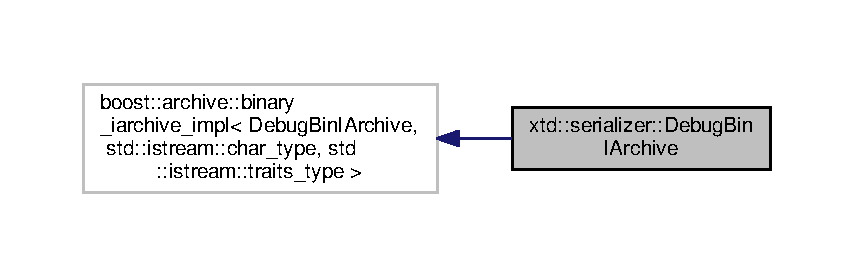
\includegraphics[width=350pt]{classxtd_1_1serializer_1_1DebugBinIArchive__inherit__graph}
\end{center}
\end{figure}


Collaboration diagram for xtd\+:\+:serializer\+:\+:Debug\+Bin\+I\+Archive\+:
\nopagebreak
\begin{figure}[H]
\begin{center}
\leavevmode
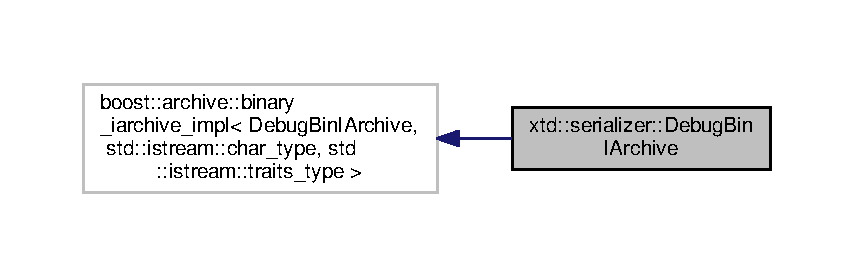
\includegraphics[width=350pt]{classxtd_1_1serializer_1_1DebugBinIArchive__coll__graph}
\end{center}
\end{figure}
\subsection*{Public Member Functions}
\begin{DoxyCompactItemize}
\item 
\hyperlink{classxtd_1_1serializer_1_1DebugBinIArchive_a4ea7040c4449afdc0a3559e2b7bc6625}{Debug\+Bin\+I\+Archive} (std\+::istream \&p\+\_\+os, int p\+\_\+flags=0)
\item 
{\footnotesize template$<$class T $>$ }\\\hyperlink{classxtd_1_1serializer_1_1DebugBinIArchive}{Debug\+Bin\+I\+Archive} \& \hyperlink{classxtd_1_1serializer_1_1DebugBinIArchive_a14ea4c855993c582b1bfd9a2c6528384}{operator$\ast$} (T \&p\+\_\+value)
\item 
{\footnotesize template$<$class T $>$ }\\\hyperlink{classxtd_1_1serializer_1_1DebugBinIArchive}{Debug\+Bin\+I\+Archive} \& \hyperlink{classxtd_1_1serializer_1_1DebugBinIArchive_a16c6f8a7cfaf497756c3edbfa16b9c0c}{operator/} (T \&p\+\_\+value)
\item 
bool \hyperlink{classxtd_1_1serializer_1_1DebugBinIArchive_a94745bb397fc67967d2ec07dc84d8c7e}{get\+Debug\+State} (void) const 
\end{DoxyCompactItemize}
\subsection*{Friends}
\begin{DoxyCompactItemize}
\item 
class \hyperlink{classxtd_1_1serializer_1_1DebugBinIArchive_aace6c76e9b138089c32705b6ec13b0e5}{boost\+::archive\+::detail\+::interface\+\_\+iarchive$<$ Debug\+Bin\+I\+Archive $>$}
\item 
class \hyperlink{classxtd_1_1serializer_1_1DebugBinIArchive_abc4efd1d58236e3dbfef39240b5457d4}{boost\+::archive\+::basic\+\_\+binary\+\_\+iarchive$<$ Debug\+Bin\+I\+Archive $>$}
\item 
class \hyperlink{classxtd_1_1serializer_1_1DebugBinIArchive_aaca003bb8a4fc59424e4025130da4edd}{boost\+::archive\+::save\+\_\+access}
\end{DoxyCompactItemize}


\subsection{Detailed Description}


Definition at line 262 of file Debug\+Archive.\+hh.



\subsection{Constructor \& Destructor Documentation}
\index{xtd\+::serializer\+::\+Debug\+Bin\+I\+Archive@{xtd\+::serializer\+::\+Debug\+Bin\+I\+Archive}!Debug\+Bin\+I\+Archive@{Debug\+Bin\+I\+Archive}}
\index{Debug\+Bin\+I\+Archive@{Debug\+Bin\+I\+Archive}!xtd\+::serializer\+::\+Debug\+Bin\+I\+Archive@{xtd\+::serializer\+::\+Debug\+Bin\+I\+Archive}}
\subsubsection[{\texorpdfstring{Debug\+Bin\+I\+Archive(std\+::istream \&p\+\_\+os, int p\+\_\+flags=0)}{DebugBinIArchive(std::istream &p_os, int p_flags=0)}}]{\setlength{\rightskip}{0pt plus 5cm}xtd\+::serializer\+::\+Debug\+Bin\+I\+Archive\+::\+Debug\+Bin\+I\+Archive (
\begin{DoxyParamCaption}
\item[{std\+::istream \&}]{p\+\_\+os, }
\item[{int}]{p\+\_\+flags = {\ttfamily 0}}
\end{DoxyParamCaption}
)\hspace{0.3cm}{\ttfamily [inline]}}\hypertarget{classxtd_1_1serializer_1_1DebugBinIArchive_a4ea7040c4449afdc0a3559e2b7bc6625}{}\label{classxtd_1_1serializer_1_1DebugBinIArchive_a4ea7040c4449afdc0a3559e2b7bc6625}


Definition at line 270 of file Debug\+Archive.\+hh.


\begin{DoxyCode}
270                                                       :
271     base(p\_os, p\_flags),
272     m\_debugMode(\textcolor{keyword}{false}),
273     m\_statusLoaded(\textcolor{keyword}{false})
274   \{\}
\end{DoxyCode}


\subsection{Member Function Documentation}
\index{xtd\+::serializer\+::\+Debug\+Bin\+I\+Archive@{xtd\+::serializer\+::\+Debug\+Bin\+I\+Archive}!get\+Debug\+State@{get\+Debug\+State}}
\index{get\+Debug\+State@{get\+Debug\+State}!xtd\+::serializer\+::\+Debug\+Bin\+I\+Archive@{xtd\+::serializer\+::\+Debug\+Bin\+I\+Archive}}
\subsubsection[{\texorpdfstring{get\+Debug\+State(void) const }{getDebugState(void) const }}]{\setlength{\rightskip}{0pt plus 5cm}bool xtd\+::serializer\+::\+Debug\+Bin\+I\+Archive\+::get\+Debug\+State (
\begin{DoxyParamCaption}
\item[{void}]{}
\end{DoxyParamCaption}
) const\hspace{0.3cm}{\ttfamily [inline]}}\hypertarget{classxtd_1_1serializer_1_1DebugBinIArchive_a94745bb397fc67967d2ec07dc84d8c7e}{}\label{classxtd_1_1serializer_1_1DebugBinIArchive_a94745bb397fc67967d2ec07dc84d8c7e}


Definition at line 300 of file Debug\+Archive.\+hh.


\begin{DoxyCode}
301   \{
302     \textcolor{keywordflow}{return} m\_debugMode;
303   \}
\end{DoxyCode}
\index{xtd\+::serializer\+::\+Debug\+Bin\+I\+Archive@{xtd\+::serializer\+::\+Debug\+Bin\+I\+Archive}!operator$\ast$@{operator$\ast$}}
\index{operator$\ast$@{operator$\ast$}!xtd\+::serializer\+::\+Debug\+Bin\+I\+Archive@{xtd\+::serializer\+::\+Debug\+Bin\+I\+Archive}}
\subsubsection[{\texorpdfstring{operator$\ast$(\+T \&p\+\_\+value)}{operator*(T &p_value)}}]{\setlength{\rightskip}{0pt plus 5cm}template$<$class T $>$ {\bf Debug\+Bin\+I\+Archive}\& xtd\+::serializer\+::\+Debug\+Bin\+I\+Archive\+::operator$\ast$ (
\begin{DoxyParamCaption}
\item[{T \&}]{p\+\_\+value}
\end{DoxyParamCaption}
)\hspace{0.3cm}{\ttfamily [inline]}}\hypertarget{classxtd_1_1serializer_1_1DebugBinIArchive_a14ea4c855993c582b1bfd9a2c6528384}{}\label{classxtd_1_1serializer_1_1DebugBinIArchive_a14ea4c855993c582b1bfd9a2c6528384}


Definition at line 277 of file Debug\+Archive.\+hh.


\begin{DoxyCode}
278   \{
279     \textcolor{keywordflow}{if} (\textcolor{keyword}{false} == m\_statusLoaded)
280     \{
281       \textcolor{comment}{//std::cout << "loading debug status..." << std::endl;}
282       base::operator&(boost::serialization::make\_nvp(\textcolor{stringliteral}{"debug"}, m\_debugMode));
283       m\_statusLoaded = \textcolor{keyword}{true};
284     \}
285     \textcolor{keywordflow}{return} base::operator&(p\_value);
286   \}
\end{DoxyCode}
\index{xtd\+::serializer\+::\+Debug\+Bin\+I\+Archive@{xtd\+::serializer\+::\+Debug\+Bin\+I\+Archive}!operator/@{operator/}}
\index{operator/@{operator/}!xtd\+::serializer\+::\+Debug\+Bin\+I\+Archive@{xtd\+::serializer\+::\+Debug\+Bin\+I\+Archive}}
\subsubsection[{\texorpdfstring{operator/(\+T \&p\+\_\+value)}{operator/(T &p_value)}}]{\setlength{\rightskip}{0pt plus 5cm}template$<$class T $>$ {\bf Debug\+Bin\+I\+Archive}\& xtd\+::serializer\+::\+Debug\+Bin\+I\+Archive\+::operator/ (
\begin{DoxyParamCaption}
\item[{T \&}]{p\+\_\+value}
\end{DoxyParamCaption}
)\hspace{0.3cm}{\ttfamily [inline]}}\hypertarget{classxtd_1_1serializer_1_1DebugBinIArchive_a16c6f8a7cfaf497756c3edbfa16b9c0c}{}\label{classxtd_1_1serializer_1_1DebugBinIArchive_a16c6f8a7cfaf497756c3edbfa16b9c0c}


Definition at line 289 of file Debug\+Archive.\+hh.


\begin{DoxyCode}
290   \{
291     \textcolor{comment}{//std::cout << "should load debug field ?" << std::endl;}
292     \textcolor{keywordflow}{if} (m\_debugMode)
293     \{
294       \textcolor{comment}{//std::cout << "loading debug field..." << std::endl;}
295       *\textcolor{keyword}{this} * p\_value;
296     \}
297     \textcolor{keywordflow}{return} *\textcolor{keyword}{this};
298   \}
\end{DoxyCode}


\subsection{Friends And Related Function Documentation}
\index{xtd\+::serializer\+::\+Debug\+Bin\+I\+Archive@{xtd\+::serializer\+::\+Debug\+Bin\+I\+Archive}!boost\+::archive\+::basic\+\_\+binary\+\_\+iarchive$<$ Debug\+Bin\+I\+Archive $>$@{boost\+::archive\+::basic\+\_\+binary\+\_\+iarchive$<$ Debug\+Bin\+I\+Archive $>$}}
\index{boost\+::archive\+::basic\+\_\+binary\+\_\+iarchive$<$ Debug\+Bin\+I\+Archive $>$@{boost\+::archive\+::basic\+\_\+binary\+\_\+iarchive$<$ Debug\+Bin\+I\+Archive $>$}!xtd\+::serializer\+::\+Debug\+Bin\+I\+Archive@{xtd\+::serializer\+::\+Debug\+Bin\+I\+Archive}}
\subsubsection[{\texorpdfstring{boost\+::archive\+::basic\+\_\+binary\+\_\+iarchive$<$ Debug\+Bin\+I\+Archive $>$}{boost::archive::basic_binary_iarchive< DebugBinIArchive >}}]{\setlength{\rightskip}{0pt plus 5cm}friend class boost\+::archive\+::basic\+\_\+binary\+\_\+iarchive$<$ {\bf Debug\+Bin\+I\+Archive} $>$\hspace{0.3cm}{\ttfamily [friend]}}\hypertarget{classxtd_1_1serializer_1_1DebugBinIArchive_abc4efd1d58236e3dbfef39240b5457d4}{}\label{classxtd_1_1serializer_1_1DebugBinIArchive_abc4efd1d58236e3dbfef39240b5457d4}


Definition at line 266 of file Debug\+Archive.\+hh.

\index{xtd\+::serializer\+::\+Debug\+Bin\+I\+Archive@{xtd\+::serializer\+::\+Debug\+Bin\+I\+Archive}!boost\+::archive\+::detail\+::interface\+\_\+iarchive$<$ Debug\+Bin\+I\+Archive $>$@{boost\+::archive\+::detail\+::interface\+\_\+iarchive$<$ Debug\+Bin\+I\+Archive $>$}}
\index{boost\+::archive\+::detail\+::interface\+\_\+iarchive$<$ Debug\+Bin\+I\+Archive $>$@{boost\+::archive\+::detail\+::interface\+\_\+iarchive$<$ Debug\+Bin\+I\+Archive $>$}!xtd\+::serializer\+::\+Debug\+Bin\+I\+Archive@{xtd\+::serializer\+::\+Debug\+Bin\+I\+Archive}}
\subsubsection[{\texorpdfstring{boost\+::archive\+::detail\+::interface\+\_\+iarchive$<$ Debug\+Bin\+I\+Archive $>$}{boost::archive::detail::interface_iarchive< DebugBinIArchive >}}]{\setlength{\rightskip}{0pt plus 5cm}friend class boost\+::archive\+::detail\+::interface\+\_\+iarchive$<$ {\bf Debug\+Bin\+I\+Archive} $>$\hspace{0.3cm}{\ttfamily [friend]}}\hypertarget{classxtd_1_1serializer_1_1DebugBinIArchive_aace6c76e9b138089c32705b6ec13b0e5}{}\label{classxtd_1_1serializer_1_1DebugBinIArchive_aace6c76e9b138089c32705b6ec13b0e5}


Definition at line 265 of file Debug\+Archive.\+hh.

\index{xtd\+::serializer\+::\+Debug\+Bin\+I\+Archive@{xtd\+::serializer\+::\+Debug\+Bin\+I\+Archive}!boost\+::archive\+::save\+\_\+access@{boost\+::archive\+::save\+\_\+access}}
\index{boost\+::archive\+::save\+\_\+access@{boost\+::archive\+::save\+\_\+access}!xtd\+::serializer\+::\+Debug\+Bin\+I\+Archive@{xtd\+::serializer\+::\+Debug\+Bin\+I\+Archive}}
\subsubsection[{\texorpdfstring{boost\+::archive\+::save\+\_\+access}{boost::archive::save_access}}]{\setlength{\rightskip}{0pt plus 5cm}friend class boost\+::archive\+::save\+\_\+access\hspace{0.3cm}{\ttfamily [friend]}}\hypertarget{classxtd_1_1serializer_1_1DebugBinIArchive_aaca003bb8a4fc59424e4025130da4edd}{}\label{classxtd_1_1serializer_1_1DebugBinIArchive_aaca003bb8a4fc59424e4025130da4edd}


Definition at line 267 of file Debug\+Archive.\+hh.



The documentation for this class was generated from the following file\+:\begin{DoxyCompactItemize}
\item 
/home/psyco/dev/xtdcpp/serializer/src/archives/\hyperlink{DebugArchive_8hh}{Debug\+Archive.\+hh}\end{DoxyCompactItemize}

\hypertarget{classxtd_1_1serializer_1_1DebugBinOArchive}{\section{xtd\-:\-:serializer\-:\-:Debug\-Bin\-O\-Archive Class Reference}
\label{classxtd_1_1serializer_1_1DebugBinOArchive}\index{xtd\-::serializer\-::\-Debug\-Bin\-O\-Archive@{xtd\-::serializer\-::\-Debug\-Bin\-O\-Archive}}
}


{\ttfamily \#include $<$Debug\-Archive.\-hh$>$}



Inheritance diagram for xtd\-:\-:serializer\-:\-:Debug\-Bin\-O\-Archive\-:
\nopagebreak
\begin{figure}[H]
\begin{center}
\leavevmode
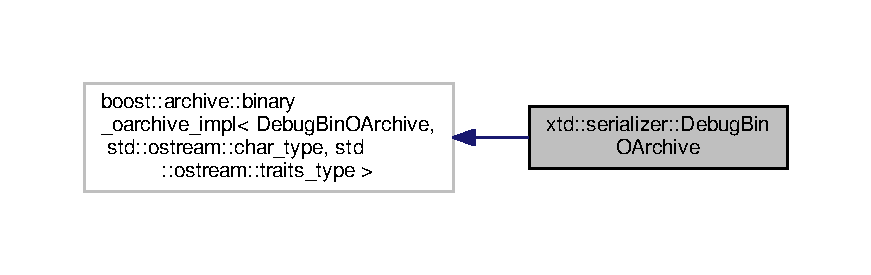
\includegraphics[width=350pt]{classxtd_1_1serializer_1_1DebugBinOArchive__inherit__graph}
\end{center}
\end{figure}


Collaboration diagram for xtd\-:\-:serializer\-:\-:Debug\-Bin\-O\-Archive\-:
\nopagebreak
\begin{figure}[H]
\begin{center}
\leavevmode
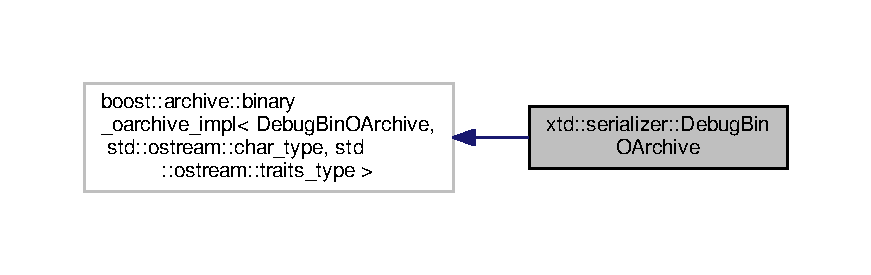
\includegraphics[width=350pt]{classxtd_1_1serializer_1_1DebugBinOArchive__coll__graph}
\end{center}
\end{figure}
\subsection*{Public Member Functions}
\begin{DoxyCompactItemize}
\item 
\hyperlink{classxtd_1_1serializer_1_1DebugBinOArchive_a24ef5240df842821499a32be217018ac}{Debug\-Bin\-O\-Archive} (std\-::ostream \&p\-\_\-os, bool p\-\_\-debug\-State=false, int p\-\_\-flags=0)
\item 
{\footnotesize template$<$class T $>$ }\\\hyperlink{classxtd_1_1serializer_1_1DebugBinOArchive}{Debug\-Bin\-O\-Archive} \& \hyperlink{classxtd_1_1serializer_1_1DebugBinOArchive_a47872bf2656b80e613d1b6d946437be2}{operator$\ast$} (T \&p\-\_\-value)
\item 
{\footnotesize template$<$class T $>$ }\\\hyperlink{classxtd_1_1serializer_1_1DebugBinOArchive}{Debug\-Bin\-O\-Archive} \& \hyperlink{classxtd_1_1serializer_1_1DebugBinOArchive_a6312cd274de08133d15bcda75d61762e}{operator/} (T \&p\-\_\-value)
\end{DoxyCompactItemize}
\subsection*{Friends}
\begin{DoxyCompactItemize}
\item 
class \hyperlink{classxtd_1_1serializer_1_1DebugBinOArchive_a8319d9e2864d97444125a3c4701611a2}{boost\-::archive\-::detail\-::interface\-\_\-oarchive$<$ Debug\-Bin\-O\-Archive $>$}
\item 
class \hyperlink{classxtd_1_1serializer_1_1DebugBinOArchive_a7b9f0abe54deccaffaf59bd14a6f9f53}{boost\-::archive\-::basic\-\_\-binary\-\_\-oarchive$<$ Debug\-Bin\-O\-Archive $>$}
\item 
class \hyperlink{classxtd_1_1serializer_1_1DebugBinOArchive_aaca003bb8a4fc59424e4025130da4edd}{boost\-::archive\-::save\-\_\-access}
\end{DoxyCompactItemize}


\subsection{Detailed Description}


Definition at line 215 of file Debug\-Archive.\-hh.



\subsection{Constructor \& Destructor Documentation}
\hypertarget{classxtd_1_1serializer_1_1DebugBinOArchive_a24ef5240df842821499a32be217018ac}{\index{xtd\-::serializer\-::\-Debug\-Bin\-O\-Archive@{xtd\-::serializer\-::\-Debug\-Bin\-O\-Archive}!Debug\-Bin\-O\-Archive@{Debug\-Bin\-O\-Archive}}
\index{Debug\-Bin\-O\-Archive@{Debug\-Bin\-O\-Archive}!xtd::serializer::DebugBinOArchive@{xtd\-::serializer\-::\-Debug\-Bin\-O\-Archive}}
\subsubsection[{Debug\-Bin\-O\-Archive}]{\setlength{\rightskip}{0pt plus 5cm}xtd\-::serializer\-::\-Debug\-Bin\-O\-Archive\-::\-Debug\-Bin\-O\-Archive (
\begin{DoxyParamCaption}
\item[{std\-::ostream \&}]{p\-\_\-os, }
\item[{bool}]{p\-\_\-debug\-State = {\ttfamily false}, }
\item[{int}]{p\-\_\-flags = {\ttfamily 0}}
\end{DoxyParamCaption}
)\hspace{0.3cm}{\ttfamily [inline]}}}\label{classxtd_1_1serializer_1_1DebugBinOArchive_a24ef5240df842821499a32be217018ac}


Definition at line 224 of file Debug\-Archive.\-hh.


\begin{DoxyCode}
224                                                                                  :
225     base(p\_os, p\_flags),
226     m\_debugMode(p\_debugState),
227     m\_statusSaved(\textcolor{keyword}{false})
228   \{\}
\end{DoxyCode}


\subsection{Member Function Documentation}
\hypertarget{classxtd_1_1serializer_1_1DebugBinOArchive_a47872bf2656b80e613d1b6d946437be2}{\index{xtd\-::serializer\-::\-Debug\-Bin\-O\-Archive@{xtd\-::serializer\-::\-Debug\-Bin\-O\-Archive}!operator$\ast$@{operator$\ast$}}
\index{operator$\ast$@{operator$\ast$}!xtd::serializer::DebugBinOArchive@{xtd\-::serializer\-::\-Debug\-Bin\-O\-Archive}}
\subsubsection[{operator$\ast$}]{\setlength{\rightskip}{0pt plus 5cm}template$<$class T $>$ {\bf Debug\-Bin\-O\-Archive}\& xtd\-::serializer\-::\-Debug\-Bin\-O\-Archive\-::operator$\ast$ (
\begin{DoxyParamCaption}
\item[{T \&}]{p\-\_\-value}
\end{DoxyParamCaption}
)\hspace{0.3cm}{\ttfamily [inline]}}}\label{classxtd_1_1serializer_1_1DebugBinOArchive_a47872bf2656b80e613d1b6d946437be2}


Definition at line 232 of file Debug\-Archive.\-hh.


\begin{DoxyCode}
233   \{
234     \textcolor{keywordflow}{if} (\textcolor{keyword}{false} == m\_statusSaved)
235     \{
236       \textcolor{comment}{//std::cout << "saving debug status..." << std::endl;}
237       base::operator&(boost::serialization::make\_nvp(\textcolor{stringliteral}{"debug"}, m\_debugMode));
238       m\_statusSaved = \textcolor{keyword}{true};
239     \}
240     \textcolor{keywordflow}{return} base::operator&(p\_value);
241   \}
\end{DoxyCode}
\hypertarget{classxtd_1_1serializer_1_1DebugBinOArchive_a6312cd274de08133d15bcda75d61762e}{\index{xtd\-::serializer\-::\-Debug\-Bin\-O\-Archive@{xtd\-::serializer\-::\-Debug\-Bin\-O\-Archive}!operator/@{operator/}}
\index{operator/@{operator/}!xtd::serializer::DebugBinOArchive@{xtd\-::serializer\-::\-Debug\-Bin\-O\-Archive}}
\subsubsection[{operator/}]{\setlength{\rightskip}{0pt plus 5cm}template$<$class T $>$ {\bf Debug\-Bin\-O\-Archive}\& xtd\-::serializer\-::\-Debug\-Bin\-O\-Archive\-::operator/ (
\begin{DoxyParamCaption}
\item[{T \&}]{p\-\_\-value}
\end{DoxyParamCaption}
)\hspace{0.3cm}{\ttfamily [inline]}}}\label{classxtd_1_1serializer_1_1DebugBinOArchive_a6312cd274de08133d15bcda75d61762e}


Definition at line 244 of file Debug\-Archive.\-hh.


\begin{DoxyCode}
245   \{
246     \textcolor{comment}{//std::cout << "should save debug field ?" << std::endl;}
247     \textcolor{keywordflow}{if} (m\_debugMode)
248     \{
249       \textcolor{comment}{//std::cout << "saving debug field..." << std::endl;}
250       *\textcolor{keyword}{this} * p\_value;
251     \}
252     \textcolor{keywordflow}{return} *\textcolor{keyword}{this};
253   \}
\end{DoxyCode}


\subsection{Friends And Related Function Documentation}
\hypertarget{classxtd_1_1serializer_1_1DebugBinOArchive_a7b9f0abe54deccaffaf59bd14a6f9f53}{\index{xtd\-::serializer\-::\-Debug\-Bin\-O\-Archive@{xtd\-::serializer\-::\-Debug\-Bin\-O\-Archive}!boost\-::archive\-::basic\-\_\-binary\-\_\-oarchive$<$ Debug\-Bin\-O\-Archive $>$@{boost\-::archive\-::basic\-\_\-binary\-\_\-oarchive$<$ Debug\-Bin\-O\-Archive $>$}}
\index{boost\-::archive\-::basic\-\_\-binary\-\_\-oarchive$<$ Debug\-Bin\-O\-Archive $>$@{boost\-::archive\-::basic\-\_\-binary\-\_\-oarchive$<$ Debug\-Bin\-O\-Archive $>$}!xtd::serializer::DebugBinOArchive@{xtd\-::serializer\-::\-Debug\-Bin\-O\-Archive}}
\subsubsection[{boost\-::archive\-::basic\-\_\-binary\-\_\-oarchive$<$ Debug\-Bin\-O\-Archive $>$}]{\setlength{\rightskip}{0pt plus 5cm}friend class boost\-::archive\-::basic\-\_\-binary\-\_\-oarchive$<$ {\bf Debug\-Bin\-O\-Archive} $>$\hspace{0.3cm}{\ttfamily [friend]}}}\label{classxtd_1_1serializer_1_1DebugBinOArchive_a7b9f0abe54deccaffaf59bd14a6f9f53}


Definition at line 220 of file Debug\-Archive.\-hh.

\hypertarget{classxtd_1_1serializer_1_1DebugBinOArchive_a8319d9e2864d97444125a3c4701611a2}{\index{xtd\-::serializer\-::\-Debug\-Bin\-O\-Archive@{xtd\-::serializer\-::\-Debug\-Bin\-O\-Archive}!boost\-::archive\-::detail\-::interface\-\_\-oarchive$<$ Debug\-Bin\-O\-Archive $>$@{boost\-::archive\-::detail\-::interface\-\_\-oarchive$<$ Debug\-Bin\-O\-Archive $>$}}
\index{boost\-::archive\-::detail\-::interface\-\_\-oarchive$<$ Debug\-Bin\-O\-Archive $>$@{boost\-::archive\-::detail\-::interface\-\_\-oarchive$<$ Debug\-Bin\-O\-Archive $>$}!xtd::serializer::DebugBinOArchive@{xtd\-::serializer\-::\-Debug\-Bin\-O\-Archive}}
\subsubsection[{boost\-::archive\-::detail\-::interface\-\_\-oarchive$<$ Debug\-Bin\-O\-Archive $>$}]{\setlength{\rightskip}{0pt plus 5cm}friend class boost\-::archive\-::detail\-::interface\-\_\-oarchive$<$ {\bf Debug\-Bin\-O\-Archive} $>$\hspace{0.3cm}{\ttfamily [friend]}}}\label{classxtd_1_1serializer_1_1DebugBinOArchive_a8319d9e2864d97444125a3c4701611a2}


Definition at line 219 of file Debug\-Archive.\-hh.

\hypertarget{classxtd_1_1serializer_1_1DebugBinOArchive_aaca003bb8a4fc59424e4025130da4edd}{\index{xtd\-::serializer\-::\-Debug\-Bin\-O\-Archive@{xtd\-::serializer\-::\-Debug\-Bin\-O\-Archive}!boost\-::archive\-::save\-\_\-access@{boost\-::archive\-::save\-\_\-access}}
\index{boost\-::archive\-::save\-\_\-access@{boost\-::archive\-::save\-\_\-access}!xtd::serializer::DebugBinOArchive@{xtd\-::serializer\-::\-Debug\-Bin\-O\-Archive}}
\subsubsection[{boost\-::archive\-::save\-\_\-access}]{\setlength{\rightskip}{0pt plus 5cm}friend class boost\-::archive\-::save\-\_\-access\hspace{0.3cm}{\ttfamily [friend]}}}\label{classxtd_1_1serializer_1_1DebugBinOArchive_aaca003bb8a4fc59424e4025130da4edd}


Definition at line 221 of file Debug\-Archive.\-hh.



The documentation for this class was generated from the following file\-:\begin{DoxyCompactItemize}
\item 
/home/travis/build/psycofdj/xtdcpp/serializer/src/archives/\hyperlink{DebugArchive_8hh}{Debug\-Archive.\-hh}\end{DoxyCompactItemize}

\hypertarget{classxtd_1_1serializer_1_1DebugTextIArchive}{\section{xtd\-:\-:serializer\-:\-:Debug\-Text\-I\-Archive Class Reference}
\label{classxtd_1_1serializer_1_1DebugTextIArchive}\index{xtd\-::serializer\-::\-Debug\-Text\-I\-Archive@{xtd\-::serializer\-::\-Debug\-Text\-I\-Archive}}
}


{\ttfamily \#include $<$Debug\-Archive.\-hh$>$}



Inheritance diagram for xtd\-:\-:serializer\-:\-:Debug\-Text\-I\-Archive\-:
\nopagebreak
\begin{figure}[H]
\begin{center}
\leavevmode
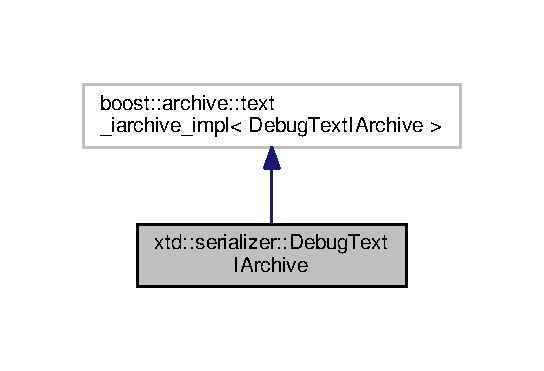
\includegraphics[width=260pt]{classxtd_1_1serializer_1_1DebugTextIArchive__inherit__graph}
\end{center}
\end{figure}


Collaboration diagram for xtd\-:\-:serializer\-:\-:Debug\-Text\-I\-Archive\-:
\nopagebreak
\begin{figure}[H]
\begin{center}
\leavevmode
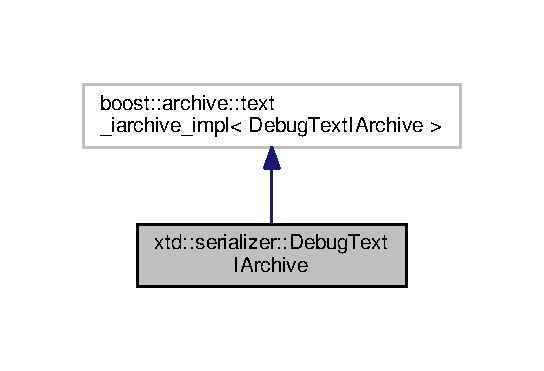
\includegraphics[width=260pt]{classxtd_1_1serializer_1_1DebugTextIArchive__coll__graph}
\end{center}
\end{figure}
\subsection*{Public Member Functions}
\begin{DoxyCompactItemize}
\item 
\hyperlink{classxtd_1_1serializer_1_1DebugTextIArchive_a97b036aced6a2612a505bca126b8e4da}{Debug\-Text\-I\-Archive} (std\-::istream \&p\-\_\-os, int p\-\_\-flags=0)
\item 
{\footnotesize template$<$class T $>$ }\\\hyperlink{classxtd_1_1serializer_1_1DebugTextIArchive}{Debug\-Text\-I\-Archive} \& \hyperlink{classxtd_1_1serializer_1_1DebugTextIArchive_a7fb53e65348749bad9e2b945b03c1e9a}{operator$\ast$} (T \&p\-\_\-value)
\item 
{\footnotesize template$<$class T $>$ }\\\hyperlink{classxtd_1_1serializer_1_1DebugTextIArchive}{Debug\-Text\-I\-Archive} \& \hyperlink{classxtd_1_1serializer_1_1DebugTextIArchive_a8c9fb4b382705609a5cd1570c63818f1}{operator/} (T \&p\-\_\-value)
\item 
bool \hyperlink{classxtd_1_1serializer_1_1DebugTextIArchive_a3ad42e3b468f60546bc76b21247ee0ca}{get\-Debug\-State} (void) const 
\end{DoxyCompactItemize}
\subsection*{Friends}
\begin{DoxyCompactItemize}
\item 
class \hyperlink{classxtd_1_1serializer_1_1DebugTextIArchive_af9e30d7c11da39f8fdf5fd8c21e4e831}{boost\-::archive\-::detail\-::interface\-\_\-iarchive$<$ Debug\-Text\-I\-Archive $>$}
\item 
class \hyperlink{classxtd_1_1serializer_1_1DebugTextIArchive_a6fe2ce7d54600795abdea507c1270a7a}{boost\-::archive\-::basic\-\_\-text\-\_\-iarchive$<$ Debug\-Text\-I\-Archive $>$}
\item 
class \hyperlink{classxtd_1_1serializer_1_1DebugTextIArchive_aaca003bb8a4fc59424e4025130da4edd}{boost\-::archive\-::save\-\_\-access}
\end{DoxyCompactItemize}


\subsection{Detailed Description}


Definition at line 165 of file Debug\-Archive.\-hh.



\subsection{Constructor \& Destructor Documentation}
\hypertarget{classxtd_1_1serializer_1_1DebugTextIArchive_a97b036aced6a2612a505bca126b8e4da}{\index{xtd\-::serializer\-::\-Debug\-Text\-I\-Archive@{xtd\-::serializer\-::\-Debug\-Text\-I\-Archive}!Debug\-Text\-I\-Archive@{Debug\-Text\-I\-Archive}}
\index{Debug\-Text\-I\-Archive@{Debug\-Text\-I\-Archive}!xtd::serializer::DebugTextIArchive@{xtd\-::serializer\-::\-Debug\-Text\-I\-Archive}}
\subsubsection[{Debug\-Text\-I\-Archive}]{\setlength{\rightskip}{0pt plus 5cm}xtd\-::serializer\-::\-Debug\-Text\-I\-Archive\-::\-Debug\-Text\-I\-Archive (
\begin{DoxyParamCaption}
\item[{std\-::istream \&}]{p\-\_\-os, }
\item[{int}]{p\-\_\-flags = {\ttfamily 0}}
\end{DoxyParamCaption}
)\hspace{0.3cm}{\ttfamily [inline]}}}\label{classxtd_1_1serializer_1_1DebugTextIArchive_a97b036aced6a2612a505bca126b8e4da}


Definition at line 173 of file Debug\-Archive.\-hh.


\begin{DoxyCode}
173                                                        :
174     base(p\_os, p\_flags),
175     m\_debugMode(\textcolor{keyword}{false}),
176     m\_statusLoaded(\textcolor{keyword}{false})
177   \{\}
\end{DoxyCode}


\subsection{Member Function Documentation}
\hypertarget{classxtd_1_1serializer_1_1DebugTextIArchive_a3ad42e3b468f60546bc76b21247ee0ca}{\index{xtd\-::serializer\-::\-Debug\-Text\-I\-Archive@{xtd\-::serializer\-::\-Debug\-Text\-I\-Archive}!get\-Debug\-State@{get\-Debug\-State}}
\index{get\-Debug\-State@{get\-Debug\-State}!xtd::serializer::DebugTextIArchive@{xtd\-::serializer\-::\-Debug\-Text\-I\-Archive}}
\subsubsection[{get\-Debug\-State}]{\setlength{\rightskip}{0pt plus 5cm}bool xtd\-::serializer\-::\-Debug\-Text\-I\-Archive\-::get\-Debug\-State (
\begin{DoxyParamCaption}
\item[{void}]{}
\end{DoxyParamCaption}
) const\hspace{0.3cm}{\ttfamily [inline]}}}\label{classxtd_1_1serializer_1_1DebugTextIArchive_a3ad42e3b468f60546bc76b21247ee0ca}


Definition at line 203 of file Debug\-Archive.\-hh.


\begin{DoxyCode}
204   \{
205     \textcolor{keywordflow}{return} m\_debugMode;
206   \}
\end{DoxyCode}
\hypertarget{classxtd_1_1serializer_1_1DebugTextIArchive_a7fb53e65348749bad9e2b945b03c1e9a}{\index{xtd\-::serializer\-::\-Debug\-Text\-I\-Archive@{xtd\-::serializer\-::\-Debug\-Text\-I\-Archive}!operator$\ast$@{operator$\ast$}}
\index{operator$\ast$@{operator$\ast$}!xtd::serializer::DebugTextIArchive@{xtd\-::serializer\-::\-Debug\-Text\-I\-Archive}}
\subsubsection[{operator$\ast$}]{\setlength{\rightskip}{0pt plus 5cm}template$<$class T $>$ {\bf Debug\-Text\-I\-Archive}\& xtd\-::serializer\-::\-Debug\-Text\-I\-Archive\-::operator$\ast$ (
\begin{DoxyParamCaption}
\item[{T \&}]{p\-\_\-value}
\end{DoxyParamCaption}
)\hspace{0.3cm}{\ttfamily [inline]}}}\label{classxtd_1_1serializer_1_1DebugTextIArchive_a7fb53e65348749bad9e2b945b03c1e9a}


Definition at line 180 of file Debug\-Archive.\-hh.


\begin{DoxyCode}
181   \{
182     \textcolor{keywordflow}{if} (\textcolor{keyword}{false} == m\_statusLoaded)
183     \{
184       \textcolor{comment}{//std::cout << "loading debug status..." << std::endl;}
185       base::operator&(boost::serialization::make\_nvp(\textcolor{stringliteral}{"debug"}, m\_debugMode));
186       m\_statusLoaded = \textcolor{keyword}{true};
187     \}
188     \textcolor{keywordflow}{return} base::operator&(p\_value);
189   \}
\end{DoxyCode}
\hypertarget{classxtd_1_1serializer_1_1DebugTextIArchive_a8c9fb4b382705609a5cd1570c63818f1}{\index{xtd\-::serializer\-::\-Debug\-Text\-I\-Archive@{xtd\-::serializer\-::\-Debug\-Text\-I\-Archive}!operator/@{operator/}}
\index{operator/@{operator/}!xtd::serializer::DebugTextIArchive@{xtd\-::serializer\-::\-Debug\-Text\-I\-Archive}}
\subsubsection[{operator/}]{\setlength{\rightskip}{0pt plus 5cm}template$<$class T $>$ {\bf Debug\-Text\-I\-Archive}\& xtd\-::serializer\-::\-Debug\-Text\-I\-Archive\-::operator/ (
\begin{DoxyParamCaption}
\item[{T \&}]{p\-\_\-value}
\end{DoxyParamCaption}
)\hspace{0.3cm}{\ttfamily [inline]}}}\label{classxtd_1_1serializer_1_1DebugTextIArchive_a8c9fb4b382705609a5cd1570c63818f1}


Definition at line 192 of file Debug\-Archive.\-hh.


\begin{DoxyCode}
193   \{
194     \textcolor{comment}{//std::cout << "should load debug field ?" << std::endl;}
195     \textcolor{keywordflow}{if} (m\_debugMode)
196     \{
197       \textcolor{comment}{//std::cout << "loading debug field..." << std::endl;}
198       *\textcolor{keyword}{this} * p\_value;
199     \}
200     \textcolor{keywordflow}{return} *\textcolor{keyword}{this};
201   \}
\end{DoxyCode}


\subsection{Friends And Related Function Documentation}
\hypertarget{classxtd_1_1serializer_1_1DebugTextIArchive_a6fe2ce7d54600795abdea507c1270a7a}{\index{xtd\-::serializer\-::\-Debug\-Text\-I\-Archive@{xtd\-::serializer\-::\-Debug\-Text\-I\-Archive}!boost\-::archive\-::basic\-\_\-text\-\_\-iarchive$<$ Debug\-Text\-I\-Archive $>$@{boost\-::archive\-::basic\-\_\-text\-\_\-iarchive$<$ Debug\-Text\-I\-Archive $>$}}
\index{boost\-::archive\-::basic\-\_\-text\-\_\-iarchive$<$ Debug\-Text\-I\-Archive $>$@{boost\-::archive\-::basic\-\_\-text\-\_\-iarchive$<$ Debug\-Text\-I\-Archive $>$}!xtd::serializer::DebugTextIArchive@{xtd\-::serializer\-::\-Debug\-Text\-I\-Archive}}
\subsubsection[{boost\-::archive\-::basic\-\_\-text\-\_\-iarchive$<$ Debug\-Text\-I\-Archive $>$}]{\setlength{\rightskip}{0pt plus 5cm}friend class boost\-::archive\-::basic\-\_\-text\-\_\-iarchive$<$ {\bf Debug\-Text\-I\-Archive} $>$\hspace{0.3cm}{\ttfamily [friend]}}}\label{classxtd_1_1serializer_1_1DebugTextIArchive_a6fe2ce7d54600795abdea507c1270a7a}


Definition at line 169 of file Debug\-Archive.\-hh.

\hypertarget{classxtd_1_1serializer_1_1DebugTextIArchive_af9e30d7c11da39f8fdf5fd8c21e4e831}{\index{xtd\-::serializer\-::\-Debug\-Text\-I\-Archive@{xtd\-::serializer\-::\-Debug\-Text\-I\-Archive}!boost\-::archive\-::detail\-::interface\-\_\-iarchive$<$ Debug\-Text\-I\-Archive $>$@{boost\-::archive\-::detail\-::interface\-\_\-iarchive$<$ Debug\-Text\-I\-Archive $>$}}
\index{boost\-::archive\-::detail\-::interface\-\_\-iarchive$<$ Debug\-Text\-I\-Archive $>$@{boost\-::archive\-::detail\-::interface\-\_\-iarchive$<$ Debug\-Text\-I\-Archive $>$}!xtd::serializer::DebugTextIArchive@{xtd\-::serializer\-::\-Debug\-Text\-I\-Archive}}
\subsubsection[{boost\-::archive\-::detail\-::interface\-\_\-iarchive$<$ Debug\-Text\-I\-Archive $>$}]{\setlength{\rightskip}{0pt plus 5cm}friend class boost\-::archive\-::detail\-::interface\-\_\-iarchive$<$ {\bf Debug\-Text\-I\-Archive} $>$\hspace{0.3cm}{\ttfamily [friend]}}}\label{classxtd_1_1serializer_1_1DebugTextIArchive_af9e30d7c11da39f8fdf5fd8c21e4e831}


Definition at line 168 of file Debug\-Archive.\-hh.

\hypertarget{classxtd_1_1serializer_1_1DebugTextIArchive_aaca003bb8a4fc59424e4025130da4edd}{\index{xtd\-::serializer\-::\-Debug\-Text\-I\-Archive@{xtd\-::serializer\-::\-Debug\-Text\-I\-Archive}!boost\-::archive\-::save\-\_\-access@{boost\-::archive\-::save\-\_\-access}}
\index{boost\-::archive\-::save\-\_\-access@{boost\-::archive\-::save\-\_\-access}!xtd::serializer::DebugTextIArchive@{xtd\-::serializer\-::\-Debug\-Text\-I\-Archive}}
\subsubsection[{boost\-::archive\-::save\-\_\-access}]{\setlength{\rightskip}{0pt plus 5cm}friend class boost\-::archive\-::save\-\_\-access\hspace{0.3cm}{\ttfamily [friend]}}}\label{classxtd_1_1serializer_1_1DebugTextIArchive_aaca003bb8a4fc59424e4025130da4edd}


Definition at line 170 of file Debug\-Archive.\-hh.



The documentation for this class was generated from the following file\-:\begin{DoxyCompactItemize}
\item 
/home/travis/build/psycofdj/xtdcpp/serializer/src/archives/\hyperlink{DebugArchive_8hh}{Debug\-Archive.\-hh}\end{DoxyCompactItemize}

\hypertarget{classxtd_1_1serializer_1_1DebugTextOArchive}{}\section{xtd\+:\+:serializer\+:\+:Debug\+Text\+O\+Archive Class Reference}
\label{classxtd_1_1serializer_1_1DebugTextOArchive}\index{xtd\+::serializer\+::\+Debug\+Text\+O\+Archive@{xtd\+::serializer\+::\+Debug\+Text\+O\+Archive}}


{\ttfamily \#include $<$Debug\+Archive.\+hh$>$}



Inheritance diagram for xtd\+:\+:serializer\+:\+:Debug\+Text\+O\+Archive\+:
\nopagebreak
\begin{figure}[H]
\begin{center}
\leavevmode
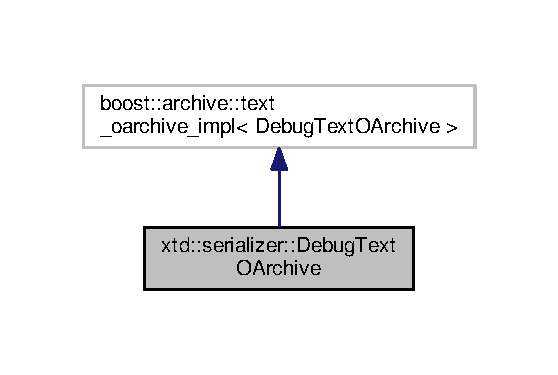
\includegraphics[width=268pt]{classxtd_1_1serializer_1_1DebugTextOArchive__inherit__graph}
\end{center}
\end{figure}


Collaboration diagram for xtd\+:\+:serializer\+:\+:Debug\+Text\+O\+Archive\+:
\nopagebreak
\begin{figure}[H]
\begin{center}
\leavevmode
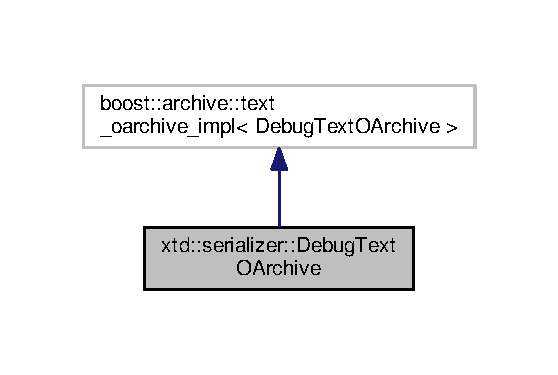
\includegraphics[width=268pt]{classxtd_1_1serializer_1_1DebugTextOArchive__coll__graph}
\end{center}
\end{figure}
\subsection*{Public Member Functions}
\begin{DoxyCompactItemize}
\item 
\hyperlink{classxtd_1_1serializer_1_1DebugTextOArchive_ac8705c1c468911d8b0c74b29156a8b8e}{Debug\+Text\+O\+Archive} (std\+::ostream \&p\+\_\+os, bool p\+\_\+debug\+State=false, int p\+\_\+flags=0)
\item 
{\footnotesize template$<$class T $>$ }\\\hyperlink{classxtd_1_1serializer_1_1DebugTextOArchive}{Debug\+Text\+O\+Archive} \& \hyperlink{classxtd_1_1serializer_1_1DebugTextOArchive_a03483bda8da712cbd5f789bcd3c20659}{operator$\ast$} (T \&p\+\_\+value)
\item 
{\footnotesize template$<$class T $>$ }\\\hyperlink{classxtd_1_1serializer_1_1DebugTextOArchive}{Debug\+Text\+O\+Archive} \& \hyperlink{classxtd_1_1serializer_1_1DebugTextOArchive_ab5bd315f1a6d164814d0ae28fca9ab1d}{operator/} (T \&p\+\_\+value)
\end{DoxyCompactItemize}
\subsection*{Friends}
\begin{DoxyCompactItemize}
\item 
class \hyperlink{classxtd_1_1serializer_1_1DebugTextOArchive_a162d16419084090d0d406eb1f23dfa6d}{boost\+::archive\+::detail\+::interface\+\_\+oarchive$<$ Debug\+Text\+O\+Archive $>$}
\item 
class \hyperlink{classxtd_1_1serializer_1_1DebugTextOArchive_ac712c773113f2ae2a71ee1f638877ab2}{boost\+::archive\+::basic\+\_\+text\+\_\+oarchive$<$ Debug\+Text\+O\+Archive $>$}
\item 
class \hyperlink{classxtd_1_1serializer_1_1DebugTextOArchive_aaca003bb8a4fc59424e4025130da4edd}{boost\+::archive\+::save\+\_\+access}
\end{DoxyCompactItemize}


\subsection{Detailed Description}


Definition at line 120 of file Debug\+Archive.\+hh.



\subsection{Constructor \& Destructor Documentation}
\index{xtd\+::serializer\+::\+Debug\+Text\+O\+Archive@{xtd\+::serializer\+::\+Debug\+Text\+O\+Archive}!Debug\+Text\+O\+Archive@{Debug\+Text\+O\+Archive}}
\index{Debug\+Text\+O\+Archive@{Debug\+Text\+O\+Archive}!xtd\+::serializer\+::\+Debug\+Text\+O\+Archive@{xtd\+::serializer\+::\+Debug\+Text\+O\+Archive}}
\subsubsection[{\texorpdfstring{Debug\+Text\+O\+Archive(std\+::ostream \&p\+\_\+os, bool p\+\_\+debug\+State=false, int p\+\_\+flags=0)}{DebugTextOArchive(std::ostream &p_os, bool p_debugState=false, int p_flags=0)}}]{\setlength{\rightskip}{0pt plus 5cm}xtd\+::serializer\+::\+Debug\+Text\+O\+Archive\+::\+Debug\+Text\+O\+Archive (
\begin{DoxyParamCaption}
\item[{std\+::ostream \&}]{p\+\_\+os, }
\item[{bool}]{p\+\_\+debug\+State = {\ttfamily false}, }
\item[{int}]{p\+\_\+flags = {\ttfamily 0}}
\end{DoxyParamCaption}
)\hspace{0.3cm}{\ttfamily [inline]}}\hypertarget{classxtd_1_1serializer_1_1DebugTextOArchive_ac8705c1c468911d8b0c74b29156a8b8e}{}\label{classxtd_1_1serializer_1_1DebugTextOArchive_ac8705c1c468911d8b0c74b29156a8b8e}


Definition at line 128 of file Debug\+Archive.\+hh.


\begin{DoxyCode}
128                                                                                   :
129     base(p\_os, p\_flags),
130     m\_debugMode(p\_debugState),
131     m\_statusSaved(\textcolor{keyword}{false})
132   \{\}
\end{DoxyCode}


\subsection{Member Function Documentation}
\index{xtd\+::serializer\+::\+Debug\+Text\+O\+Archive@{xtd\+::serializer\+::\+Debug\+Text\+O\+Archive}!operator$\ast$@{operator$\ast$}}
\index{operator$\ast$@{operator$\ast$}!xtd\+::serializer\+::\+Debug\+Text\+O\+Archive@{xtd\+::serializer\+::\+Debug\+Text\+O\+Archive}}
\subsubsection[{\texorpdfstring{operator$\ast$(\+T \&p\+\_\+value)}{operator*(T &p_value)}}]{\setlength{\rightskip}{0pt plus 5cm}template$<$class T $>$ {\bf Debug\+Text\+O\+Archive}\& xtd\+::serializer\+::\+Debug\+Text\+O\+Archive\+::operator$\ast$ (
\begin{DoxyParamCaption}
\item[{T \&}]{p\+\_\+value}
\end{DoxyParamCaption}
)\hspace{0.3cm}{\ttfamily [inline]}}\hypertarget{classxtd_1_1serializer_1_1DebugTextOArchive_a03483bda8da712cbd5f789bcd3c20659}{}\label{classxtd_1_1serializer_1_1DebugTextOArchive_a03483bda8da712cbd5f789bcd3c20659}


Definition at line 136 of file Debug\+Archive.\+hh.


\begin{DoxyCode}
137   \{
138     \textcolor{keywordflow}{if} (\textcolor{keyword}{false} == m\_statusSaved)
139     \{
140       \textcolor{comment}{//std::cout << "saving debug status..." << std::endl;}
141       base::operator&(boost::serialization::make\_nvp(\textcolor{stringliteral}{"debug"}, m\_debugMode));
142       m\_statusSaved = \textcolor{keyword}{true};
143     \}
144     \textcolor{keywordflow}{return} base::operator&(p\_value);
145   \}
\end{DoxyCode}
\index{xtd\+::serializer\+::\+Debug\+Text\+O\+Archive@{xtd\+::serializer\+::\+Debug\+Text\+O\+Archive}!operator/@{operator/}}
\index{operator/@{operator/}!xtd\+::serializer\+::\+Debug\+Text\+O\+Archive@{xtd\+::serializer\+::\+Debug\+Text\+O\+Archive}}
\subsubsection[{\texorpdfstring{operator/(\+T \&p\+\_\+value)}{operator/(T &p_value)}}]{\setlength{\rightskip}{0pt plus 5cm}template$<$class T $>$ {\bf Debug\+Text\+O\+Archive}\& xtd\+::serializer\+::\+Debug\+Text\+O\+Archive\+::operator/ (
\begin{DoxyParamCaption}
\item[{T \&}]{p\+\_\+value}
\end{DoxyParamCaption}
)\hspace{0.3cm}{\ttfamily [inline]}}\hypertarget{classxtd_1_1serializer_1_1DebugTextOArchive_ab5bd315f1a6d164814d0ae28fca9ab1d}{}\label{classxtd_1_1serializer_1_1DebugTextOArchive_ab5bd315f1a6d164814d0ae28fca9ab1d}


Definition at line 148 of file Debug\+Archive.\+hh.


\begin{DoxyCode}
149   \{
150     \textcolor{comment}{//std::cout << "should save debug field ?" << std::endl;}
151     \textcolor{keywordflow}{if} (m\_debugMode)
152     \{
153       \textcolor{comment}{//std::cout << "saving debug field..." << std::endl;}
154       *\textcolor{keyword}{this} * p\_value;
155     \}
156     \textcolor{keywordflow}{return} *\textcolor{keyword}{this};
157   \}
\end{DoxyCode}


\subsection{Friends And Related Function Documentation}
\index{xtd\+::serializer\+::\+Debug\+Text\+O\+Archive@{xtd\+::serializer\+::\+Debug\+Text\+O\+Archive}!boost\+::archive\+::basic\+\_\+text\+\_\+oarchive$<$ Debug\+Text\+O\+Archive $>$@{boost\+::archive\+::basic\+\_\+text\+\_\+oarchive$<$ Debug\+Text\+O\+Archive $>$}}
\index{boost\+::archive\+::basic\+\_\+text\+\_\+oarchive$<$ Debug\+Text\+O\+Archive $>$@{boost\+::archive\+::basic\+\_\+text\+\_\+oarchive$<$ Debug\+Text\+O\+Archive $>$}!xtd\+::serializer\+::\+Debug\+Text\+O\+Archive@{xtd\+::serializer\+::\+Debug\+Text\+O\+Archive}}
\subsubsection[{\texorpdfstring{boost\+::archive\+::basic\+\_\+text\+\_\+oarchive$<$ Debug\+Text\+O\+Archive $>$}{boost::archive::basic_text_oarchive< DebugTextOArchive >}}]{\setlength{\rightskip}{0pt plus 5cm}friend class boost\+::archive\+::basic\+\_\+text\+\_\+oarchive$<$ {\bf Debug\+Text\+O\+Archive} $>$\hspace{0.3cm}{\ttfamily [friend]}}\hypertarget{classxtd_1_1serializer_1_1DebugTextOArchive_ac712c773113f2ae2a71ee1f638877ab2}{}\label{classxtd_1_1serializer_1_1DebugTextOArchive_ac712c773113f2ae2a71ee1f638877ab2}


Definition at line 124 of file Debug\+Archive.\+hh.

\index{xtd\+::serializer\+::\+Debug\+Text\+O\+Archive@{xtd\+::serializer\+::\+Debug\+Text\+O\+Archive}!boost\+::archive\+::detail\+::interface\+\_\+oarchive$<$ Debug\+Text\+O\+Archive $>$@{boost\+::archive\+::detail\+::interface\+\_\+oarchive$<$ Debug\+Text\+O\+Archive $>$}}
\index{boost\+::archive\+::detail\+::interface\+\_\+oarchive$<$ Debug\+Text\+O\+Archive $>$@{boost\+::archive\+::detail\+::interface\+\_\+oarchive$<$ Debug\+Text\+O\+Archive $>$}!xtd\+::serializer\+::\+Debug\+Text\+O\+Archive@{xtd\+::serializer\+::\+Debug\+Text\+O\+Archive}}
\subsubsection[{\texorpdfstring{boost\+::archive\+::detail\+::interface\+\_\+oarchive$<$ Debug\+Text\+O\+Archive $>$}{boost::archive::detail::interface_oarchive< DebugTextOArchive >}}]{\setlength{\rightskip}{0pt plus 5cm}friend class boost\+::archive\+::detail\+::interface\+\_\+oarchive$<$ {\bf Debug\+Text\+O\+Archive} $>$\hspace{0.3cm}{\ttfamily [friend]}}\hypertarget{classxtd_1_1serializer_1_1DebugTextOArchive_a162d16419084090d0d406eb1f23dfa6d}{}\label{classxtd_1_1serializer_1_1DebugTextOArchive_a162d16419084090d0d406eb1f23dfa6d}


Definition at line 123 of file Debug\+Archive.\+hh.

\index{xtd\+::serializer\+::\+Debug\+Text\+O\+Archive@{xtd\+::serializer\+::\+Debug\+Text\+O\+Archive}!boost\+::archive\+::save\+\_\+access@{boost\+::archive\+::save\+\_\+access}}
\index{boost\+::archive\+::save\+\_\+access@{boost\+::archive\+::save\+\_\+access}!xtd\+::serializer\+::\+Debug\+Text\+O\+Archive@{xtd\+::serializer\+::\+Debug\+Text\+O\+Archive}}
\subsubsection[{\texorpdfstring{boost\+::archive\+::save\+\_\+access}{boost::archive::save_access}}]{\setlength{\rightskip}{0pt plus 5cm}friend class boost\+::archive\+::save\+\_\+access\hspace{0.3cm}{\ttfamily [friend]}}\hypertarget{classxtd_1_1serializer_1_1DebugTextOArchive_aaca003bb8a4fc59424e4025130da4edd}{}\label{classxtd_1_1serializer_1_1DebugTextOArchive_aaca003bb8a4fc59424e4025130da4edd}


Definition at line 125 of file Debug\+Archive.\+hh.



The documentation for this class was generated from the following file\+:\begin{DoxyCompactItemize}
\item 
/home/psyco/dev/xtdcpp/serializer/src/archives/\hyperlink{DebugArchive_8hh}{Debug\+Archive.\+hh}\end{DoxyCompactItemize}

\hypertarget{classxtd_1_1serializer_1_1DebugXmlIArchive}{}\section{xtd\+:\+:serializer\+:\+:Debug\+Xml\+I\+Archive Class Reference}
\label{classxtd_1_1serializer_1_1DebugXmlIArchive}\index{xtd\+::serializer\+::\+Debug\+Xml\+I\+Archive@{xtd\+::serializer\+::\+Debug\+Xml\+I\+Archive}}


{\ttfamily \#include $<$Debug\+Archive.\+hh$>$}



Inheritance diagram for xtd\+:\+:serializer\+:\+:Debug\+Xml\+I\+Archive\+:
\nopagebreak
\begin{figure}[H]
\begin{center}
\leavevmode
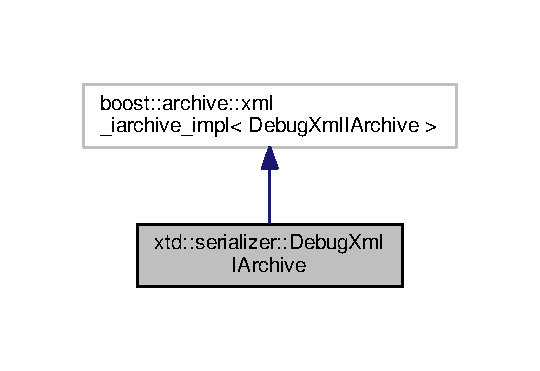
\includegraphics[width=259pt]{classxtd_1_1serializer_1_1DebugXmlIArchive__inherit__graph}
\end{center}
\end{figure}


Collaboration diagram for xtd\+:\+:serializer\+:\+:Debug\+Xml\+I\+Archive\+:
\nopagebreak
\begin{figure}[H]
\begin{center}
\leavevmode
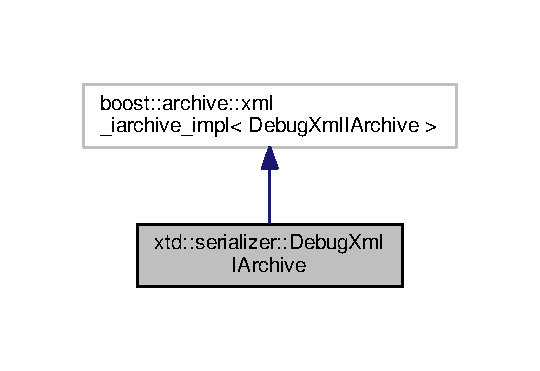
\includegraphics[width=259pt]{classxtd_1_1serializer_1_1DebugXmlIArchive__coll__graph}
\end{center}
\end{figure}
\subsection*{Public Member Functions}
\begin{DoxyCompactItemize}
\item 
\hyperlink{classxtd_1_1serializer_1_1DebugXmlIArchive_a877cd247551b625bec79846a8b9274d1}{Debug\+Xml\+I\+Archive} (std\+::istream \&p\+\_\+os, int p\+\_\+flags=0)
\item 
{\footnotesize template$<$class T $>$ }\\\hyperlink{classxtd_1_1serializer_1_1DebugXmlIArchive}{Debug\+Xml\+I\+Archive} \& \hyperlink{classxtd_1_1serializer_1_1DebugXmlIArchive_a40060fc623b46cb0332a7ea56b1d9148}{operator$\ast$} (T \&p\+\_\+value)
\item 
{\footnotesize template$<$class T $>$ }\\\hyperlink{classxtd_1_1serializer_1_1DebugXmlIArchive}{Debug\+Xml\+I\+Archive} \& \hyperlink{classxtd_1_1serializer_1_1DebugXmlIArchive_a523764ab4e37ba9cb07dc7d7269ca507}{operator/} (T \&p\+\_\+value)
\item 
bool \hyperlink{classxtd_1_1serializer_1_1DebugXmlIArchive_a40860da9e1a849931364d86b56557357}{get\+Debug\+State} (void) const 
\end{DoxyCompactItemize}
\subsection*{Friends}
\begin{DoxyCompactItemize}
\item 
class \hyperlink{classxtd_1_1serializer_1_1DebugXmlIArchive_a54f75e33da74496cd06e608f4bec85dc}{boost\+::archive\+::detail\+::interface\+\_\+iarchive$<$ Debug\+Xml\+I\+Archive $>$}
\item 
class \hyperlink{classxtd_1_1serializer_1_1DebugXmlIArchive_a54affbd4684171cc9e5cabf2db73ffe5}{boost\+::archive\+::basic\+\_\+xml\+\_\+iarchive$<$ Debug\+Xml\+I\+Archive $>$}
\item 
class \hyperlink{classxtd_1_1serializer_1_1DebugXmlIArchive_aaca003bb8a4fc59424e4025130da4edd}{boost\+::archive\+::save\+\_\+access}
\end{DoxyCompactItemize}


\subsection{Detailed Description}


Definition at line 70 of file Debug\+Archive.\+hh.



\subsection{Constructor \& Destructor Documentation}
\index{xtd\+::serializer\+::\+Debug\+Xml\+I\+Archive@{xtd\+::serializer\+::\+Debug\+Xml\+I\+Archive}!Debug\+Xml\+I\+Archive@{Debug\+Xml\+I\+Archive}}
\index{Debug\+Xml\+I\+Archive@{Debug\+Xml\+I\+Archive}!xtd\+::serializer\+::\+Debug\+Xml\+I\+Archive@{xtd\+::serializer\+::\+Debug\+Xml\+I\+Archive}}
\subsubsection[{\texorpdfstring{Debug\+Xml\+I\+Archive(std\+::istream \&p\+\_\+os, int p\+\_\+flags=0)}{DebugXmlIArchive(std::istream &p_os, int p_flags=0)}}]{\setlength{\rightskip}{0pt plus 5cm}xtd\+::serializer\+::\+Debug\+Xml\+I\+Archive\+::\+Debug\+Xml\+I\+Archive (
\begin{DoxyParamCaption}
\item[{std\+::istream \&}]{p\+\_\+os, }
\item[{int}]{p\+\_\+flags = {\ttfamily 0}}
\end{DoxyParamCaption}
)\hspace{0.3cm}{\ttfamily [inline]}}\hypertarget{classxtd_1_1serializer_1_1DebugXmlIArchive_a877cd247551b625bec79846a8b9274d1}{}\label{classxtd_1_1serializer_1_1DebugXmlIArchive_a877cd247551b625bec79846a8b9274d1}


Definition at line 78 of file Debug\+Archive.\+hh.


\begin{DoxyCode}
78                                                       :
79     base(p\_os, p\_flags),
80     m\_debugMode(\textcolor{keyword}{false}),
81     m\_statusLoaded(\textcolor{keyword}{false})
82   \{\}
\end{DoxyCode}


\subsection{Member Function Documentation}
\index{xtd\+::serializer\+::\+Debug\+Xml\+I\+Archive@{xtd\+::serializer\+::\+Debug\+Xml\+I\+Archive}!get\+Debug\+State@{get\+Debug\+State}}
\index{get\+Debug\+State@{get\+Debug\+State}!xtd\+::serializer\+::\+Debug\+Xml\+I\+Archive@{xtd\+::serializer\+::\+Debug\+Xml\+I\+Archive}}
\subsubsection[{\texorpdfstring{get\+Debug\+State(void) const }{getDebugState(void) const }}]{\setlength{\rightskip}{0pt plus 5cm}bool xtd\+::serializer\+::\+Debug\+Xml\+I\+Archive\+::get\+Debug\+State (
\begin{DoxyParamCaption}
\item[{void}]{}
\end{DoxyParamCaption}
) const\hspace{0.3cm}{\ttfamily [inline]}}\hypertarget{classxtd_1_1serializer_1_1DebugXmlIArchive_a40860da9e1a849931364d86b56557357}{}\label{classxtd_1_1serializer_1_1DebugXmlIArchive_a40860da9e1a849931364d86b56557357}


Definition at line 108 of file Debug\+Archive.\+hh.


\begin{DoxyCode}
109   \{
110     \textcolor{keywordflow}{return} m\_debugMode;
111   \}
\end{DoxyCode}
\index{xtd\+::serializer\+::\+Debug\+Xml\+I\+Archive@{xtd\+::serializer\+::\+Debug\+Xml\+I\+Archive}!operator$\ast$@{operator$\ast$}}
\index{operator$\ast$@{operator$\ast$}!xtd\+::serializer\+::\+Debug\+Xml\+I\+Archive@{xtd\+::serializer\+::\+Debug\+Xml\+I\+Archive}}
\subsubsection[{\texorpdfstring{operator$\ast$(\+T \&p\+\_\+value)}{operator*(T &p_value)}}]{\setlength{\rightskip}{0pt plus 5cm}template$<$class T $>$ {\bf Debug\+Xml\+I\+Archive}\& xtd\+::serializer\+::\+Debug\+Xml\+I\+Archive\+::operator$\ast$ (
\begin{DoxyParamCaption}
\item[{T \&}]{p\+\_\+value}
\end{DoxyParamCaption}
)\hspace{0.3cm}{\ttfamily [inline]}}\hypertarget{classxtd_1_1serializer_1_1DebugXmlIArchive_a40060fc623b46cb0332a7ea56b1d9148}{}\label{classxtd_1_1serializer_1_1DebugXmlIArchive_a40060fc623b46cb0332a7ea56b1d9148}


Definition at line 85 of file Debug\+Archive.\+hh.


\begin{DoxyCode}
86   \{
87     \textcolor{keywordflow}{if} (\textcolor{keyword}{false} == m\_statusLoaded)
88     \{
89       \textcolor{comment}{//std::cout << "loading debug status..." << std::endl;}
90       base::operator&(boost::serialization::make\_nvp(\textcolor{stringliteral}{"debug"}, m\_debugMode));
91       m\_statusLoaded = \textcolor{keyword}{true};
92     \}
93     \textcolor{keywordflow}{return} base::operator&(p\_value);
94   \}
\end{DoxyCode}
\index{xtd\+::serializer\+::\+Debug\+Xml\+I\+Archive@{xtd\+::serializer\+::\+Debug\+Xml\+I\+Archive}!operator/@{operator/}}
\index{operator/@{operator/}!xtd\+::serializer\+::\+Debug\+Xml\+I\+Archive@{xtd\+::serializer\+::\+Debug\+Xml\+I\+Archive}}
\subsubsection[{\texorpdfstring{operator/(\+T \&p\+\_\+value)}{operator/(T &p_value)}}]{\setlength{\rightskip}{0pt plus 5cm}template$<$class T $>$ {\bf Debug\+Xml\+I\+Archive}\& xtd\+::serializer\+::\+Debug\+Xml\+I\+Archive\+::operator/ (
\begin{DoxyParamCaption}
\item[{T \&}]{p\+\_\+value}
\end{DoxyParamCaption}
)\hspace{0.3cm}{\ttfamily [inline]}}\hypertarget{classxtd_1_1serializer_1_1DebugXmlIArchive_a523764ab4e37ba9cb07dc7d7269ca507}{}\label{classxtd_1_1serializer_1_1DebugXmlIArchive_a523764ab4e37ba9cb07dc7d7269ca507}


Definition at line 97 of file Debug\+Archive.\+hh.


\begin{DoxyCode}
98   \{
99     \textcolor{comment}{//std::cout << "should load debug field ?" << std::endl;}
100     \textcolor{keywordflow}{if} (m\_debugMode)
101     \{
102       \textcolor{comment}{//std::cout << "loading debug field..." << std::endl;}
103       *\textcolor{keyword}{this} * p\_value;
104     \}
105     \textcolor{keywordflow}{return} *\textcolor{keyword}{this};
106   \}
\end{DoxyCode}


\subsection{Friends And Related Function Documentation}
\index{xtd\+::serializer\+::\+Debug\+Xml\+I\+Archive@{xtd\+::serializer\+::\+Debug\+Xml\+I\+Archive}!boost\+::archive\+::basic\+\_\+xml\+\_\+iarchive$<$ Debug\+Xml\+I\+Archive $>$@{boost\+::archive\+::basic\+\_\+xml\+\_\+iarchive$<$ Debug\+Xml\+I\+Archive $>$}}
\index{boost\+::archive\+::basic\+\_\+xml\+\_\+iarchive$<$ Debug\+Xml\+I\+Archive $>$@{boost\+::archive\+::basic\+\_\+xml\+\_\+iarchive$<$ Debug\+Xml\+I\+Archive $>$}!xtd\+::serializer\+::\+Debug\+Xml\+I\+Archive@{xtd\+::serializer\+::\+Debug\+Xml\+I\+Archive}}
\subsubsection[{\texorpdfstring{boost\+::archive\+::basic\+\_\+xml\+\_\+iarchive$<$ Debug\+Xml\+I\+Archive $>$}{boost::archive::basic_xml_iarchive< DebugXmlIArchive >}}]{\setlength{\rightskip}{0pt plus 5cm}friend class boost\+::archive\+::basic\+\_\+xml\+\_\+iarchive$<$ {\bf Debug\+Xml\+I\+Archive} $>$\hspace{0.3cm}{\ttfamily [friend]}}\hypertarget{classxtd_1_1serializer_1_1DebugXmlIArchive_a54affbd4684171cc9e5cabf2db73ffe5}{}\label{classxtd_1_1serializer_1_1DebugXmlIArchive_a54affbd4684171cc9e5cabf2db73ffe5}


Definition at line 74 of file Debug\+Archive.\+hh.

\index{xtd\+::serializer\+::\+Debug\+Xml\+I\+Archive@{xtd\+::serializer\+::\+Debug\+Xml\+I\+Archive}!boost\+::archive\+::detail\+::interface\+\_\+iarchive$<$ Debug\+Xml\+I\+Archive $>$@{boost\+::archive\+::detail\+::interface\+\_\+iarchive$<$ Debug\+Xml\+I\+Archive $>$}}
\index{boost\+::archive\+::detail\+::interface\+\_\+iarchive$<$ Debug\+Xml\+I\+Archive $>$@{boost\+::archive\+::detail\+::interface\+\_\+iarchive$<$ Debug\+Xml\+I\+Archive $>$}!xtd\+::serializer\+::\+Debug\+Xml\+I\+Archive@{xtd\+::serializer\+::\+Debug\+Xml\+I\+Archive}}
\subsubsection[{\texorpdfstring{boost\+::archive\+::detail\+::interface\+\_\+iarchive$<$ Debug\+Xml\+I\+Archive $>$}{boost::archive::detail::interface_iarchive< DebugXmlIArchive >}}]{\setlength{\rightskip}{0pt plus 5cm}friend class boost\+::archive\+::detail\+::interface\+\_\+iarchive$<$ {\bf Debug\+Xml\+I\+Archive} $>$\hspace{0.3cm}{\ttfamily [friend]}}\hypertarget{classxtd_1_1serializer_1_1DebugXmlIArchive_a54f75e33da74496cd06e608f4bec85dc}{}\label{classxtd_1_1serializer_1_1DebugXmlIArchive_a54f75e33da74496cd06e608f4bec85dc}


Definition at line 73 of file Debug\+Archive.\+hh.

\index{xtd\+::serializer\+::\+Debug\+Xml\+I\+Archive@{xtd\+::serializer\+::\+Debug\+Xml\+I\+Archive}!boost\+::archive\+::save\+\_\+access@{boost\+::archive\+::save\+\_\+access}}
\index{boost\+::archive\+::save\+\_\+access@{boost\+::archive\+::save\+\_\+access}!xtd\+::serializer\+::\+Debug\+Xml\+I\+Archive@{xtd\+::serializer\+::\+Debug\+Xml\+I\+Archive}}
\subsubsection[{\texorpdfstring{boost\+::archive\+::save\+\_\+access}{boost::archive::save_access}}]{\setlength{\rightskip}{0pt plus 5cm}friend class boost\+::archive\+::save\+\_\+access\hspace{0.3cm}{\ttfamily [friend]}}\hypertarget{classxtd_1_1serializer_1_1DebugXmlIArchive_aaca003bb8a4fc59424e4025130da4edd}{}\label{classxtd_1_1serializer_1_1DebugXmlIArchive_aaca003bb8a4fc59424e4025130da4edd}


Definition at line 75 of file Debug\+Archive.\+hh.



The documentation for this class was generated from the following file\+:\begin{DoxyCompactItemize}
\item 
/home/psyco/dev/xtdcpp/serializer/src/archives/\hyperlink{DebugArchive_8hh}{Debug\+Archive.\+hh}\end{DoxyCompactItemize}

\hypertarget{classxtd_1_1serializer_1_1DebugXmlOArchive}{}\section{xtd\+:\+:serializer\+:\+:Debug\+Xml\+O\+Archive Class Reference}
\label{classxtd_1_1serializer_1_1DebugXmlOArchive}\index{xtd\+::serializer\+::\+Debug\+Xml\+O\+Archive@{xtd\+::serializer\+::\+Debug\+Xml\+O\+Archive}}


{\ttfamily \#include $<$Debug\+Archive.\+hh$>$}



Inheritance diagram for xtd\+:\+:serializer\+:\+:Debug\+Xml\+O\+Archive\+:
\nopagebreak
\begin{figure}[H]
\begin{center}
\leavevmode
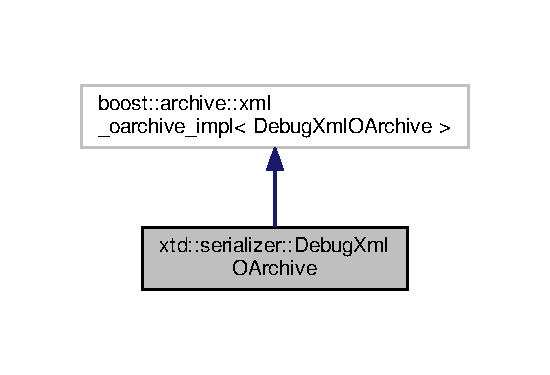
\includegraphics[width=266pt]{classxtd_1_1serializer_1_1DebugXmlOArchive__inherit__graph}
\end{center}
\end{figure}


Collaboration diagram for xtd\+:\+:serializer\+:\+:Debug\+Xml\+O\+Archive\+:
\nopagebreak
\begin{figure}[H]
\begin{center}
\leavevmode
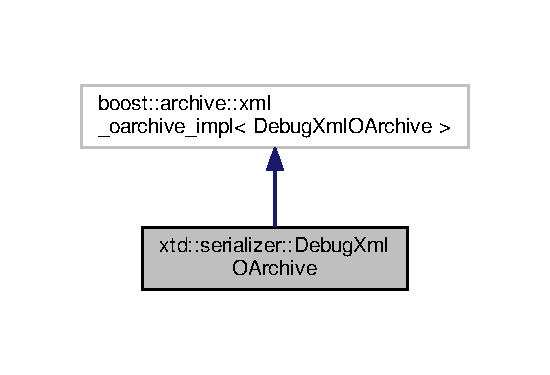
\includegraphics[width=266pt]{classxtd_1_1serializer_1_1DebugXmlOArchive__coll__graph}
\end{center}
\end{figure}
\subsection*{Public Member Functions}
\begin{DoxyCompactItemize}
\item 
\hyperlink{classxtd_1_1serializer_1_1DebugXmlOArchive_aff4ee095fcc036756c7326731a15e9b7}{Debug\+Xml\+O\+Archive} (std\+::ostream \&p\+\_\+os, bool p\+\_\+debug\+State=false, int p\+\_\+flags=0)
\item 
{\footnotesize template$<$class T $>$ }\\\hyperlink{classxtd_1_1serializer_1_1DebugXmlOArchive}{Debug\+Xml\+O\+Archive} \& \hyperlink{classxtd_1_1serializer_1_1DebugXmlOArchive_a537495d2f70d2553edf308bafd0a6327}{operator$\ast$} (T \&p\+\_\+value)
\item 
{\footnotesize template$<$class T $>$ }\\\hyperlink{classxtd_1_1serializer_1_1DebugXmlOArchive}{Debug\+Xml\+O\+Archive} \& \hyperlink{classxtd_1_1serializer_1_1DebugXmlOArchive_a8e0706fca2bb1dd85556b537db740baf}{operator/} (T \&p\+\_\+value)
\end{DoxyCompactItemize}
\subsection*{Friends}
\begin{DoxyCompactItemize}
\item 
class \hyperlink{classxtd_1_1serializer_1_1DebugXmlOArchive_ade7e327f8089db178808693b17013b37}{boost\+::archive\+::detail\+::interface\+\_\+oarchive$<$ Debug\+Xml\+O\+Archive $>$}
\item 
class \hyperlink{classxtd_1_1serializer_1_1DebugXmlOArchive_ae9a53f0a6d08579fd714365dec459e66}{boost\+::archive\+::basic\+\_\+xml\+\_\+oarchive$<$ Debug\+Xml\+O\+Archive $>$}
\item 
class \hyperlink{classxtd_1_1serializer_1_1DebugXmlOArchive_aaca003bb8a4fc59424e4025130da4edd}{boost\+::archive\+::save\+\_\+access}
\end{DoxyCompactItemize}


\subsection{Detailed Description}


Definition at line 25 of file Debug\+Archive.\+hh.



\subsection{Constructor \& Destructor Documentation}
\index{xtd\+::serializer\+::\+Debug\+Xml\+O\+Archive@{xtd\+::serializer\+::\+Debug\+Xml\+O\+Archive}!Debug\+Xml\+O\+Archive@{Debug\+Xml\+O\+Archive}}
\index{Debug\+Xml\+O\+Archive@{Debug\+Xml\+O\+Archive}!xtd\+::serializer\+::\+Debug\+Xml\+O\+Archive@{xtd\+::serializer\+::\+Debug\+Xml\+O\+Archive}}
\subsubsection[{\texorpdfstring{Debug\+Xml\+O\+Archive(std\+::ostream \&p\+\_\+os, bool p\+\_\+debug\+State=false, int p\+\_\+flags=0)}{DebugXmlOArchive(std::ostream &p_os, bool p_debugState=false, int p_flags=0)}}]{\setlength{\rightskip}{0pt plus 5cm}xtd\+::serializer\+::\+Debug\+Xml\+O\+Archive\+::\+Debug\+Xml\+O\+Archive (
\begin{DoxyParamCaption}
\item[{std\+::ostream \&}]{p\+\_\+os, }
\item[{bool}]{p\+\_\+debug\+State = {\ttfamily false}, }
\item[{int}]{p\+\_\+flags = {\ttfamily 0}}
\end{DoxyParamCaption}
)\hspace{0.3cm}{\ttfamily [inline]}}\hypertarget{classxtd_1_1serializer_1_1DebugXmlOArchive_aff4ee095fcc036756c7326731a15e9b7}{}\label{classxtd_1_1serializer_1_1DebugXmlOArchive_aff4ee095fcc036756c7326731a15e9b7}


Definition at line 33 of file Debug\+Archive.\+hh.


\begin{DoxyCode}
33                                                                                  :
34     base(p\_os, p\_flags),
35     m\_debugMode(p\_debugState),
36     m\_statusSaved(\textcolor{keyword}{false})
37   \{\}
\end{DoxyCode}


\subsection{Member Function Documentation}
\index{xtd\+::serializer\+::\+Debug\+Xml\+O\+Archive@{xtd\+::serializer\+::\+Debug\+Xml\+O\+Archive}!operator$\ast$@{operator$\ast$}}
\index{operator$\ast$@{operator$\ast$}!xtd\+::serializer\+::\+Debug\+Xml\+O\+Archive@{xtd\+::serializer\+::\+Debug\+Xml\+O\+Archive}}
\subsubsection[{\texorpdfstring{operator$\ast$(\+T \&p\+\_\+value)}{operator*(T &p_value)}}]{\setlength{\rightskip}{0pt plus 5cm}template$<$class T $>$ {\bf Debug\+Xml\+O\+Archive}\& xtd\+::serializer\+::\+Debug\+Xml\+O\+Archive\+::operator$\ast$ (
\begin{DoxyParamCaption}
\item[{T \&}]{p\+\_\+value}
\end{DoxyParamCaption}
)\hspace{0.3cm}{\ttfamily [inline]}}\hypertarget{classxtd_1_1serializer_1_1DebugXmlOArchive_a537495d2f70d2553edf308bafd0a6327}{}\label{classxtd_1_1serializer_1_1DebugXmlOArchive_a537495d2f70d2553edf308bafd0a6327}


Definition at line 41 of file Debug\+Archive.\+hh.


\begin{DoxyCode}
42   \{
43     \textcolor{keywordflow}{if} (\textcolor{keyword}{false} == m\_statusSaved)
44     \{
45       \textcolor{comment}{//std::cout << "saving debug status..." << std::endl;}
46       base::operator&(boost::serialization::make\_nvp(\textcolor{stringliteral}{"debug"}, m\_debugMode));
47       m\_statusSaved = \textcolor{keyword}{true};
48     \}
49     \textcolor{keywordflow}{return} base::operator&(p\_value);
50   \}
\end{DoxyCode}
\index{xtd\+::serializer\+::\+Debug\+Xml\+O\+Archive@{xtd\+::serializer\+::\+Debug\+Xml\+O\+Archive}!operator/@{operator/}}
\index{operator/@{operator/}!xtd\+::serializer\+::\+Debug\+Xml\+O\+Archive@{xtd\+::serializer\+::\+Debug\+Xml\+O\+Archive}}
\subsubsection[{\texorpdfstring{operator/(\+T \&p\+\_\+value)}{operator/(T &p_value)}}]{\setlength{\rightskip}{0pt plus 5cm}template$<$class T $>$ {\bf Debug\+Xml\+O\+Archive}\& xtd\+::serializer\+::\+Debug\+Xml\+O\+Archive\+::operator/ (
\begin{DoxyParamCaption}
\item[{T \&}]{p\+\_\+value}
\end{DoxyParamCaption}
)\hspace{0.3cm}{\ttfamily [inline]}}\hypertarget{classxtd_1_1serializer_1_1DebugXmlOArchive_a8e0706fca2bb1dd85556b537db740baf}{}\label{classxtd_1_1serializer_1_1DebugXmlOArchive_a8e0706fca2bb1dd85556b537db740baf}


Definition at line 53 of file Debug\+Archive.\+hh.


\begin{DoxyCode}
54   \{
55     \textcolor{comment}{//std::cout << "should save debug field ?" << std::endl;}
56     \textcolor{keywordflow}{if} (m\_debugMode)
57     \{
58       \textcolor{comment}{//std::cout << "saving debug field..." << std::endl;}
59       *\textcolor{keyword}{this} * p\_value;
60     \}
61     \textcolor{keywordflow}{return} *\textcolor{keyword}{this};
62   \}
\end{DoxyCode}


\subsection{Friends And Related Function Documentation}
\index{xtd\+::serializer\+::\+Debug\+Xml\+O\+Archive@{xtd\+::serializer\+::\+Debug\+Xml\+O\+Archive}!boost\+::archive\+::basic\+\_\+xml\+\_\+oarchive$<$ Debug\+Xml\+O\+Archive $>$@{boost\+::archive\+::basic\+\_\+xml\+\_\+oarchive$<$ Debug\+Xml\+O\+Archive $>$}}
\index{boost\+::archive\+::basic\+\_\+xml\+\_\+oarchive$<$ Debug\+Xml\+O\+Archive $>$@{boost\+::archive\+::basic\+\_\+xml\+\_\+oarchive$<$ Debug\+Xml\+O\+Archive $>$}!xtd\+::serializer\+::\+Debug\+Xml\+O\+Archive@{xtd\+::serializer\+::\+Debug\+Xml\+O\+Archive}}
\subsubsection[{\texorpdfstring{boost\+::archive\+::basic\+\_\+xml\+\_\+oarchive$<$ Debug\+Xml\+O\+Archive $>$}{boost::archive::basic_xml_oarchive< DebugXmlOArchive >}}]{\setlength{\rightskip}{0pt plus 5cm}friend class boost\+::archive\+::basic\+\_\+xml\+\_\+oarchive$<$ {\bf Debug\+Xml\+O\+Archive} $>$\hspace{0.3cm}{\ttfamily [friend]}}\hypertarget{classxtd_1_1serializer_1_1DebugXmlOArchive_ae9a53f0a6d08579fd714365dec459e66}{}\label{classxtd_1_1serializer_1_1DebugXmlOArchive_ae9a53f0a6d08579fd714365dec459e66}


Definition at line 29 of file Debug\+Archive.\+hh.

\index{xtd\+::serializer\+::\+Debug\+Xml\+O\+Archive@{xtd\+::serializer\+::\+Debug\+Xml\+O\+Archive}!boost\+::archive\+::detail\+::interface\+\_\+oarchive$<$ Debug\+Xml\+O\+Archive $>$@{boost\+::archive\+::detail\+::interface\+\_\+oarchive$<$ Debug\+Xml\+O\+Archive $>$}}
\index{boost\+::archive\+::detail\+::interface\+\_\+oarchive$<$ Debug\+Xml\+O\+Archive $>$@{boost\+::archive\+::detail\+::interface\+\_\+oarchive$<$ Debug\+Xml\+O\+Archive $>$}!xtd\+::serializer\+::\+Debug\+Xml\+O\+Archive@{xtd\+::serializer\+::\+Debug\+Xml\+O\+Archive}}
\subsubsection[{\texorpdfstring{boost\+::archive\+::detail\+::interface\+\_\+oarchive$<$ Debug\+Xml\+O\+Archive $>$}{boost::archive::detail::interface_oarchive< DebugXmlOArchive >}}]{\setlength{\rightskip}{0pt plus 5cm}friend class boost\+::archive\+::detail\+::interface\+\_\+oarchive$<$ {\bf Debug\+Xml\+O\+Archive} $>$\hspace{0.3cm}{\ttfamily [friend]}}\hypertarget{classxtd_1_1serializer_1_1DebugXmlOArchive_ade7e327f8089db178808693b17013b37}{}\label{classxtd_1_1serializer_1_1DebugXmlOArchive_ade7e327f8089db178808693b17013b37}


Definition at line 28 of file Debug\+Archive.\+hh.

\index{xtd\+::serializer\+::\+Debug\+Xml\+O\+Archive@{xtd\+::serializer\+::\+Debug\+Xml\+O\+Archive}!boost\+::archive\+::save\+\_\+access@{boost\+::archive\+::save\+\_\+access}}
\index{boost\+::archive\+::save\+\_\+access@{boost\+::archive\+::save\+\_\+access}!xtd\+::serializer\+::\+Debug\+Xml\+O\+Archive@{xtd\+::serializer\+::\+Debug\+Xml\+O\+Archive}}
\subsubsection[{\texorpdfstring{boost\+::archive\+::save\+\_\+access}{boost::archive::save_access}}]{\setlength{\rightskip}{0pt plus 5cm}friend class boost\+::archive\+::save\+\_\+access\hspace{0.3cm}{\ttfamily [friend]}}\hypertarget{classxtd_1_1serializer_1_1DebugXmlOArchive_aaca003bb8a4fc59424e4025130da4edd}{}\label{classxtd_1_1serializer_1_1DebugXmlOArchive_aaca003bb8a4fc59424e4025130da4edd}


Definition at line 30 of file Debug\+Archive.\+hh.



The documentation for this class was generated from the following file\+:\begin{DoxyCompactItemize}
\item 
/home/psyco/dev/xtdcpp/serializer/src/archives/\hyperlink{DebugArchive_8hh}{Debug\+Archive.\+hh}\end{DoxyCompactItemize}

\hypertarget{classxtd_1_1serializer_1_1Doc}{}\section{xtd\+:\+:serializer\+:\+:Doc Class Reference}
\label{classxtd_1_1serializer_1_1Doc}\index{xtd\+::serializer\+::\+Doc@{xtd\+::serializer\+::\+Doc}}


{\ttfamily \#include $<$Doc.\+hh$>$}

\subsection*{Public Types}
\begin{DoxyCompactItemize}
\item 
typedef vector$<$ \hyperlink{classxtd_1_1serializer_1_1Doc}{Doc} $>$ \hyperlink{classxtd_1_1serializer_1_1Doc_a993fd17fc627ae6d1af0aad1a11e9975}{t\+\_\+listof}
\end{DoxyCompactItemize}
\subsection*{Public Member Functions}
\begin{DoxyCompactItemize}
\item 
\hyperlink{classxtd_1_1serializer_1_1Doc_ab1d69c51eaac6754260114a91186061f}{Doc} (void)
\end{DoxyCompactItemize}
\subsection*{Public Attributes}
\begin{DoxyCompactItemize}
\item 
uint32\+\_\+t \hyperlink{classxtd_1_1serializer_1_1Doc_ac6e0a47819dac6373483fb0dd5ad91d0}{m\+\_\+score}
\item 
uint32\+\_\+t \hyperlink{classxtd_1_1serializer_1_1Doc_ae35b707444a257c668b6cc8dfb2d63e4}{m\+\_\+debug\+Score}
\end{DoxyCompactItemize}
\subsection*{Friends}
\begin{DoxyCompactItemize}
\item 
class \hyperlink{classxtd_1_1serializer_1_1Doc_ac98d07dd8f7b70e16ccb9a01abf56b9c}{boost\+::serialization\+::access}
\end{DoxyCompactItemize}


\subsection{Detailed Description}


Definition at line 10 of file Doc.\+hh.



\subsection{Member Typedef Documentation}
\index{xtd\+::serializer\+::\+Doc@{xtd\+::serializer\+::\+Doc}!t\+\_\+listof@{t\+\_\+listof}}
\index{t\+\_\+listof@{t\+\_\+listof}!xtd\+::serializer\+::\+Doc@{xtd\+::serializer\+::\+Doc}}
\subsubsection[{\texorpdfstring{t\+\_\+listof}{t_listof}}]{\setlength{\rightskip}{0pt plus 5cm}typedef vector$<${\bf Doc}$>$ {\bf xtd\+::serializer\+::\+Doc\+::t\+\_\+listof}}\hypertarget{classxtd_1_1serializer_1_1Doc_a993fd17fc627ae6d1af0aad1a11e9975}{}\label{classxtd_1_1serializer_1_1Doc_a993fd17fc627ae6d1af0aad1a11e9975}


Definition at line 15 of file Doc.\+hh.



\subsection{Constructor \& Destructor Documentation}
\index{xtd\+::serializer\+::\+Doc@{xtd\+::serializer\+::\+Doc}!Doc@{Doc}}
\index{Doc@{Doc}!xtd\+::serializer\+::\+Doc@{xtd\+::serializer\+::\+Doc}}
\subsubsection[{\texorpdfstring{Doc(void)}{Doc(void)}}]{\setlength{\rightskip}{0pt plus 5cm}xtd\+::serializer\+::\+Doc\+::\+Doc (
\begin{DoxyParamCaption}
\item[{void}]{}
\end{DoxyParamCaption}
)}\hypertarget{classxtd_1_1serializer_1_1Doc_ab1d69c51eaac6754260114a91186061f}{}\label{classxtd_1_1serializer_1_1Doc_ab1d69c51eaac6754260114a91186061f}


Definition at line 6 of file Doc.\+cc.


\begin{DoxyCode}
6              :
7   \hyperlink{classxtd_1_1serializer_1_1Doc_ac6e0a47819dac6373483fb0dd5ad91d0}{m\_score}(std::numeric\_limits<uint32\_t>::max()),
8   \hyperlink{classxtd_1_1serializer_1_1Doc_ae35b707444a257c668b6cc8dfb2d63e4}{m\_debugScore}(std::numeric\_limits<uint32\_t>::max())
9 \{
10 \}
\end{DoxyCode}


\subsection{Friends And Related Function Documentation}
\index{xtd\+::serializer\+::\+Doc@{xtd\+::serializer\+::\+Doc}!boost\+::serialization\+::access@{boost\+::serialization\+::access}}
\index{boost\+::serialization\+::access@{boost\+::serialization\+::access}!xtd\+::serializer\+::\+Doc@{xtd\+::serializer\+::\+Doc}}
\subsubsection[{\texorpdfstring{boost\+::serialization\+::access}{boost::serialization::access}}]{\setlength{\rightskip}{0pt plus 5cm}friend class boost\+::serialization\+::access\hspace{0.3cm}{\ttfamily [friend]}}\hypertarget{classxtd_1_1serializer_1_1Doc_ac98d07dd8f7b70e16ccb9a01abf56b9c}{}\label{classxtd_1_1serializer_1_1Doc_ac98d07dd8f7b70e16ccb9a01abf56b9c}


Definition at line 12 of file Doc.\+hh.



\subsection{Member Data Documentation}
\index{xtd\+::serializer\+::\+Doc@{xtd\+::serializer\+::\+Doc}!m\+\_\+debug\+Score@{m\+\_\+debug\+Score}}
\index{m\+\_\+debug\+Score@{m\+\_\+debug\+Score}!xtd\+::serializer\+::\+Doc@{xtd\+::serializer\+::\+Doc}}
\subsubsection[{\texorpdfstring{m\+\_\+debug\+Score}{m_debugScore}}]{\setlength{\rightskip}{0pt plus 5cm}uint32\+\_\+t xtd\+::serializer\+::\+Doc\+::m\+\_\+debug\+Score}\hypertarget{classxtd_1_1serializer_1_1Doc_ae35b707444a257c668b6cc8dfb2d63e4}{}\label{classxtd_1_1serializer_1_1Doc_ae35b707444a257c668b6cc8dfb2d63e4}


Definition at line 27 of file Doc.\+hh.

\index{xtd\+::serializer\+::\+Doc@{xtd\+::serializer\+::\+Doc}!m\+\_\+score@{m\+\_\+score}}
\index{m\+\_\+score@{m\+\_\+score}!xtd\+::serializer\+::\+Doc@{xtd\+::serializer\+::\+Doc}}
\subsubsection[{\texorpdfstring{m\+\_\+score}{m_score}}]{\setlength{\rightskip}{0pt plus 5cm}uint32\+\_\+t xtd\+::serializer\+::\+Doc\+::m\+\_\+score}\hypertarget{classxtd_1_1serializer_1_1Doc_ac6e0a47819dac6373483fb0dd5ad91d0}{}\label{classxtd_1_1serializer_1_1Doc_ac6e0a47819dac6373483fb0dd5ad91d0}


Definition at line 25 of file Doc.\+hh.



The documentation for this class was generated from the following files\+:\begin{DoxyCompactItemize}
\item 
/home/psyco/dev/xtdcpp/serializer/src/objects/\hyperlink{Doc_8hh}{Doc.\+hh}\item 
/home/psyco/dev/xtdcpp/serializer/src/objects/\hyperlink{Doc_8cc}{Doc.\+cc}\end{DoxyCompactItemize}

\hypertarget{structxtd_1_1serializer_1_1mode}{}\section{xtd\+:\+:serializer\+:\+:mode Struct Reference}
\label{structxtd_1_1serializer_1_1mode}\index{xtd\+::serializer\+::mode@{xtd\+::serializer\+::mode}}


{\ttfamily \#include $<$serializer.\+hh$>$}

\subsection*{Classes}
\begin{DoxyCompactItemize}
\item 
struct \hyperlink{structxtd_1_1serializer_1_1mode_1_1bin}{bin}
\item 
struct \hyperlink{structxtd_1_1serializer_1_1mode_1_1text}{text}
\item 
struct \hyperlink{structxtd_1_1serializer_1_1mode_1_1xml}{xml}
\end{DoxyCompactItemize}


\subsection{Detailed Description}


Definition at line 17 of file serializer.\+hh.



The documentation for this struct was generated from the following file\+:\begin{DoxyCompactItemize}
\item 
/home/psyco/dev/xtdcpp/serializer/src/\hyperlink{serializer_8hh}{serializer.\+hh}\end{DoxyCompactItemize}

\hypertarget{structxtd_1_1serializer_1_1option}{\section{xtd\-:\-:serializer\-:\-:option Struct Reference}
\label{structxtd_1_1serializer_1_1option}\index{xtd\-::serializer\-::option@{xtd\-::serializer\-::option}}
}


{\ttfamily \#include $<$serializer.\-hh$>$}

\subsection*{Public Member Functions}
\begin{DoxyCompactItemize}
\item 
\hyperlink{structxtd_1_1serializer_1_1option_a3c67cf48442b85d8c4224f8cf4c5d24c}{option} (void)
\item 
\hyperlink{structxtd_1_1serializer_1_1option_a32191820441da6474c53eca8599b26f1}{option} (bool p\-\_\-no\-Header, bool p\-\_\-no\-Codecvt, bool p\-\_\-no\-Xml\-Tag\-Cheking)
\item 
int \hyperlink{structxtd_1_1serializer_1_1option_a6d3cb66902f782254150e4e07cf3284c}{value} (void) const 
\end{DoxyCompactItemize}


\subsection{Detailed Description}


Definition at line 36 of file serializer.\-hh.



\subsection{Constructor \& Destructor Documentation}
\hypertarget{structxtd_1_1serializer_1_1option_a3c67cf48442b85d8c4224f8cf4c5d24c}{\index{xtd\-::serializer\-::option@{xtd\-::serializer\-::option}!option@{option}}
\index{option@{option}!xtd::serializer::option@{xtd\-::serializer\-::option}}
\subsubsection[{option}]{\setlength{\rightskip}{0pt plus 5cm}xtd\-::serializer\-::option\-::option (
\begin{DoxyParamCaption}
\item[{void}]{}
\end{DoxyParamCaption}
)\hspace{0.3cm}{\ttfamily [inline]}}}\label{structxtd_1_1serializer_1_1option_a3c67cf48442b85d8c4224f8cf4c5d24c}


Definition at line 38 of file serializer.\-hh.


\begin{DoxyCode}
38                :
39     m\_noHeader(\textcolor{keyword}{false}),
40     m\_noCodecvt(\textcolor{keyword}{false}),
41     m\_noXmlTagChecking(\textcolor{keyword}{false})
42   \{
43   \}
\end{DoxyCode}
\hypertarget{structxtd_1_1serializer_1_1option_a32191820441da6474c53eca8599b26f1}{\index{xtd\-::serializer\-::option@{xtd\-::serializer\-::option}!option@{option}}
\index{option@{option}!xtd::serializer::option@{xtd\-::serializer\-::option}}
\subsubsection[{option}]{\setlength{\rightskip}{0pt plus 5cm}xtd\-::serializer\-::option\-::option (
\begin{DoxyParamCaption}
\item[{bool}]{p\-\_\-no\-Header, }
\item[{bool}]{p\-\_\-no\-Codecvt, }
\item[{bool}]{p\-\_\-no\-Xml\-Tag\-Cheking}
\end{DoxyParamCaption}
)\hspace{0.3cm}{\ttfamily [inline]}}}\label{structxtd_1_1serializer_1_1option_a32191820441da6474c53eca8599b26f1}


Definition at line 45 of file serializer.\-hh.


\begin{DoxyCode}
45                                                                     :
46     m\_noHeader(p\_noHeader),
47     m\_noCodecvt(p\_noCodecvt),
48     m\_noXmlTagChecking(p\_noXmlTagCheking)
49   \{
50   \}
\end{DoxyCode}


\subsection{Member Function Documentation}
\hypertarget{structxtd_1_1serializer_1_1option_a6d3cb66902f782254150e4e07cf3284c}{\index{xtd\-::serializer\-::option@{xtd\-::serializer\-::option}!value@{value}}
\index{value@{value}!xtd::serializer::option@{xtd\-::serializer\-::option}}
\subsubsection[{value}]{\setlength{\rightskip}{0pt plus 5cm}int xtd\-::serializer\-::option\-::value (
\begin{DoxyParamCaption}
\item[{void}]{}
\end{DoxyParamCaption}
) const\hspace{0.3cm}{\ttfamily [inline]}}}\label{structxtd_1_1serializer_1_1option_a6d3cb66902f782254150e4e07cf3284c}


Definition at line 52 of file serializer.\-hh.


\begin{DoxyCode}
53   \{
54     \textcolor{keywordtype}{int} l\_result = 0;
55 
56     \textcolor{keywordflow}{if} (m\_noHeader)         l\_result |= boost::archive::no\_header;
57     \textcolor{keywordflow}{if} (m\_noCodecvt)        l\_result |= boost::archive::no\_codecvt;
58     \textcolor{keywordflow}{if} (m\_noXmlTagChecking) l\_result |= boost::archive::no\_xml\_tag\_checking;
59     \textcolor{keywordflow}{return} l\_result;
60   \}
\end{DoxyCode}


The documentation for this struct was generated from the following file\-:\begin{DoxyCompactItemize}
\item 
/home/travis/build/psycofdj/xtdcpp/serializer/src/\hyperlink{serializer_8hh}{serializer.\-hh}\end{DoxyCompactItemize}

\hypertarget{structxtd_1_1serializer_1_1serializer}{\section{xtd\-:\-:serializer\-:\-:serializer$<$ Mode $>$ Struct Template Reference}
\label{structxtd_1_1serializer_1_1serializer}\index{xtd\-::serializer\-::serializer$<$ Mode $>$@{xtd\-::serializer\-::serializer$<$ Mode $>$}}
}


{\ttfamily \#include $<$serializer.\-hh$>$}

\subsection*{Static Public Member Functions}
\begin{DoxyCompactItemize}
\item 
{\footnotesize template$<$class T $>$ }\\static void \hyperlink{structxtd_1_1serializer_1_1serializer_a3e2f6195fd27da1f10e131facc8e017f}{save} (std\-::ostream \&p\-\_\-stream, const T \&p\-\_\-object, bool p\-\_\-debug, \hyperlink{structxtd_1_1serializer_1_1option}{option} p\-\_\-opt=\hyperlink{structxtd_1_1serializer_1_1option}{option}())
\item 
{\footnotesize template$<$class T $>$ }\\static void \hyperlink{structxtd_1_1serializer_1_1serializer_ac8fd960ff27c165ad77f657f685add30}{load} (std\-::istream \&p\-\_\-stream, T \&p\-\_\-object, bool \&p\-\_\-debug, \hyperlink{structxtd_1_1serializer_1_1option}{option} p\-\_\-opt=\hyperlink{structxtd_1_1serializer_1_1option}{option}())
\end{DoxyCompactItemize}


\subsection{Detailed Description}
\subsubsection*{template$<$class Mode$>$struct xtd\-::serializer\-::serializer$<$ Mode $>$}



Definition at line 70 of file serializer.\-hh.



\subsection{Member Function Documentation}
\hypertarget{structxtd_1_1serializer_1_1serializer_ac8fd960ff27c165ad77f657f685add30}{\index{xtd\-::serializer\-::serializer@{xtd\-::serializer\-::serializer}!load@{load}}
\index{load@{load}!xtd::serializer::serializer@{xtd\-::serializer\-::serializer}}
\subsubsection[{load}]{\setlength{\rightskip}{0pt plus 5cm}template$<$class Mode $>$ template$<$class T $>$ static void {\bf xtd\-::serializer\-::serializer}$<$ Mode $>$\-::load (
\begin{DoxyParamCaption}
\item[{std\-::istream \&}]{p\-\_\-stream, }
\item[{T \&}]{p\-\_\-object, }
\item[{bool \&}]{p\-\_\-debug, }
\item[{{\bf option}}]{p\-\_\-opt = {\ttfamily {\bf option}()}}
\end{DoxyParamCaption}
)\hspace{0.3cm}{\ttfamily [static]}}}\label{structxtd_1_1serializer_1_1serializer_ac8fd960ff27c165ad77f657f685add30}
\hypertarget{structxtd_1_1serializer_1_1serializer_a3e2f6195fd27da1f10e131facc8e017f}{\index{xtd\-::serializer\-::serializer@{xtd\-::serializer\-::serializer}!save@{save}}
\index{save@{save}!xtd::serializer::serializer@{xtd\-::serializer\-::serializer}}
\subsubsection[{save}]{\setlength{\rightskip}{0pt plus 5cm}template$<$class Mode $>$ template$<$class T $>$ static void {\bf xtd\-::serializer\-::serializer}$<$ Mode $>$\-::save (
\begin{DoxyParamCaption}
\item[{std\-::ostream \&}]{p\-\_\-stream, }
\item[{const T \&}]{p\-\_\-object, }
\item[{bool}]{p\-\_\-debug, }
\item[{{\bf option}}]{p\-\_\-opt = {\ttfamily {\bf option}()}}
\end{DoxyParamCaption}
)\hspace{0.3cm}{\ttfamily [static]}}}\label{structxtd_1_1serializer_1_1serializer_a3e2f6195fd27da1f10e131facc8e017f}


The documentation for this struct was generated from the following file\-:\begin{DoxyCompactItemize}
\item 
/home/travis/build/psycofdj/xtdcpp/serializer/src/\hyperlink{serializer_8hh}{serializer.\-hh}\end{DoxyCompactItemize}

\hypertarget{structxtd_1_1serializer_1_1mode_1_1text}{}\section{xtd\+:\+:serializer\+:\+:mode\+:\+:text Struct Reference}
\label{structxtd_1_1serializer_1_1mode_1_1text}\index{xtd\+::serializer\+::mode\+::text@{xtd\+::serializer\+::mode\+::text}}


{\ttfamily \#include $<$serializer.\+hh$>$}

\subsection*{Public Types}
\begin{DoxyCompactItemize}
\item 
typedef \hyperlink{classxtd_1_1serializer_1_1DebugTextOArchive}{Debug\+Text\+O\+Archive} \hyperlink{structxtd_1_1serializer_1_1mode_1_1text_a8be416039df8bbed799423bb996811a8}{saver}
\item 
typedef \hyperlink{classxtd_1_1serializer_1_1DebugTextIArchive}{Debug\+Text\+I\+Archive} \hyperlink{structxtd_1_1serializer_1_1mode_1_1text_ad178828d538da6465ca47886a70ac664}{loader}
\end{DoxyCompactItemize}


\subsection{Detailed Description}


Definition at line 19 of file serializer.\+hh.



\subsection{Member Typedef Documentation}
\index{xtd\+::serializer\+::mode\+::text@{xtd\+::serializer\+::mode\+::text}!loader@{loader}}
\index{loader@{loader}!xtd\+::serializer\+::mode\+::text@{xtd\+::serializer\+::mode\+::text}}
\subsubsection[{\texorpdfstring{loader}{loader}}]{\setlength{\rightskip}{0pt plus 5cm}typedef {\bf Debug\+Text\+I\+Archive} {\bf xtd\+::serializer\+::mode\+::text\+::loader}}\hypertarget{structxtd_1_1serializer_1_1mode_1_1text_ad178828d538da6465ca47886a70ac664}{}\label{structxtd_1_1serializer_1_1mode_1_1text_ad178828d538da6465ca47886a70ac664}


Definition at line 22 of file serializer.\+hh.

\index{xtd\+::serializer\+::mode\+::text@{xtd\+::serializer\+::mode\+::text}!saver@{saver}}
\index{saver@{saver}!xtd\+::serializer\+::mode\+::text@{xtd\+::serializer\+::mode\+::text}}
\subsubsection[{\texorpdfstring{saver}{saver}}]{\setlength{\rightskip}{0pt plus 5cm}typedef {\bf Debug\+Text\+O\+Archive} {\bf xtd\+::serializer\+::mode\+::text\+::saver}}\hypertarget{structxtd_1_1serializer_1_1mode_1_1text_a8be416039df8bbed799423bb996811a8}{}\label{structxtd_1_1serializer_1_1mode_1_1text_a8be416039df8bbed799423bb996811a8}


Definition at line 21 of file serializer.\+hh.



The documentation for this struct was generated from the following file\+:\begin{DoxyCompactItemize}
\item 
/home/psyco/dev/xtdcpp/serializer/src/\hyperlink{serializer_8hh}{serializer.\+hh}\end{DoxyCompactItemize}

\hypertarget{structxtd_1_1serializer_1_1mode_1_1xml}{}\section{xtd\+:\+:serializer\+:\+:mode\+:\+:xml Struct Reference}
\label{structxtd_1_1serializer_1_1mode_1_1xml}\index{xtd\+::serializer\+::mode\+::xml@{xtd\+::serializer\+::mode\+::xml}}


{\ttfamily \#include $<$serializer.\+hh$>$}

\subsection*{Public Types}
\begin{DoxyCompactItemize}
\item 
typedef \hyperlink{classxtd_1_1serializer_1_1DebugXmlOArchive}{Debug\+Xml\+O\+Archive} \hyperlink{structxtd_1_1serializer_1_1mode_1_1xml_a630743906b9808c209a9d7bce84427bc}{saver}
\item 
typedef \hyperlink{classxtd_1_1serializer_1_1DebugXmlIArchive}{Debug\+Xml\+I\+Archive} \hyperlink{structxtd_1_1serializer_1_1mode_1_1xml_a645aca92f671ad196a17282c44a69a83}{loader}
\end{DoxyCompactItemize}


\subsection{Detailed Description}


Definition at line 24 of file serializer.\+hh.



\subsection{Member Typedef Documentation}
\index{xtd\+::serializer\+::mode\+::xml@{xtd\+::serializer\+::mode\+::xml}!loader@{loader}}
\index{loader@{loader}!xtd\+::serializer\+::mode\+::xml@{xtd\+::serializer\+::mode\+::xml}}
\subsubsection[{\texorpdfstring{loader}{loader}}]{\setlength{\rightskip}{0pt plus 5cm}typedef {\bf Debug\+Xml\+I\+Archive} {\bf xtd\+::serializer\+::mode\+::xml\+::loader}}\hypertarget{structxtd_1_1serializer_1_1mode_1_1xml_a645aca92f671ad196a17282c44a69a83}{}\label{structxtd_1_1serializer_1_1mode_1_1xml_a645aca92f671ad196a17282c44a69a83}


Definition at line 27 of file serializer.\+hh.

\index{xtd\+::serializer\+::mode\+::xml@{xtd\+::serializer\+::mode\+::xml}!saver@{saver}}
\index{saver@{saver}!xtd\+::serializer\+::mode\+::xml@{xtd\+::serializer\+::mode\+::xml}}
\subsubsection[{\texorpdfstring{saver}{saver}}]{\setlength{\rightskip}{0pt plus 5cm}typedef {\bf Debug\+Xml\+O\+Archive} {\bf xtd\+::serializer\+::mode\+::xml\+::saver}}\hypertarget{structxtd_1_1serializer_1_1mode_1_1xml_a630743906b9808c209a9d7bce84427bc}{}\label{structxtd_1_1serializer_1_1mode_1_1xml_a630743906b9808c209a9d7bce84427bc}


Definition at line 26 of file serializer.\+hh.



The documentation for this struct was generated from the following file\+:\begin{DoxyCompactItemize}
\item 
/home/psyco/dev/xtdcpp/serializer/src/\hyperlink{serializer_8hh}{serializer.\+hh}\end{DoxyCompactItemize}

\chapter{File Documentation}
\hypertarget{DebugArchive_8cc}{\section{/home/travis/build/psycofdj/xtdcpp/serializer/src/archives/\-Debug\-Archive.cc File Reference}
\label{DebugArchive_8cc}\index{/home/travis/build/psycofdj/xtdcpp/serializer/src/archives/\-Debug\-Archive.\-cc@{/home/travis/build/psycofdj/xtdcpp/serializer/src/archives/\-Debug\-Archive.\-cc}}
}
{\ttfamily \#include \char`\"{}archives/\-Debug\-Archive.\-hh\char`\"{}}\\*
{\ttfamily \#include $<$boost/archive/detail/archive\-\_\-serializer\-\_\-map.\-hpp$>$}\\*
{\ttfamily \#include $<$boost/archive/impl/archive\-\_\-serializer\-\_\-map.\-ipp$>$}\\*
{\ttfamily \#include $<$boost/archive/impl/basic\-\_\-xml\-\_\-oarchive.\-ipp$>$}\\*
{\ttfamily \#include $<$boost/archive/impl/xml\-\_\-oarchive\-\_\-impl.\-ipp$>$}\\*
{\ttfamily \#include $<$boost/archive/impl/basic\-\_\-xml\-\_\-iarchive.\-ipp$>$}\\*
{\ttfamily \#include $<$boost/archive/impl/xml\-\_\-iarchive\-\_\-impl.\-ipp$>$}\\*
{\ttfamily \#include $<$boost/archive/impl/text\-\_\-oarchive\-\_\-impl.\-ipp$>$}\\*
{\ttfamily \#include $<$boost/archive/impl/text\-\_\-iarchive\-\_\-impl.\-ipp$>$}\\*
{\ttfamily \#include $<$boost/archive/impl/basic\-\_\-binary\-\_\-oprimitive.\-ipp$>$}\\*
{\ttfamily \#include $<$boost/archive/impl/basic\-\_\-text\-\_\-oarchive.\-ipp$>$}\\*
{\ttfamily \#include $<$boost/archive/impl/basic\-\_\-binary\-\_\-oarchive.\-ipp$>$}\\*
{\ttfamily \#include $<$boost/archive/impl/basic\-\_\-binary\-\_\-iprimitive.\-ipp$>$}\\*
{\ttfamily \#include $<$boost/archive/impl/basic\-\_\-text\-\_\-iarchive.\-ipp$>$}\\*
{\ttfamily \#include $<$boost/archive/impl/basic\-\_\-binary\-\_\-iarchive.\-ipp$>$}\\*
Include dependency graph for Debug\-Archive.\-cc\-:
\nopagebreak
\begin{figure}[H]
\begin{center}
\leavevmode
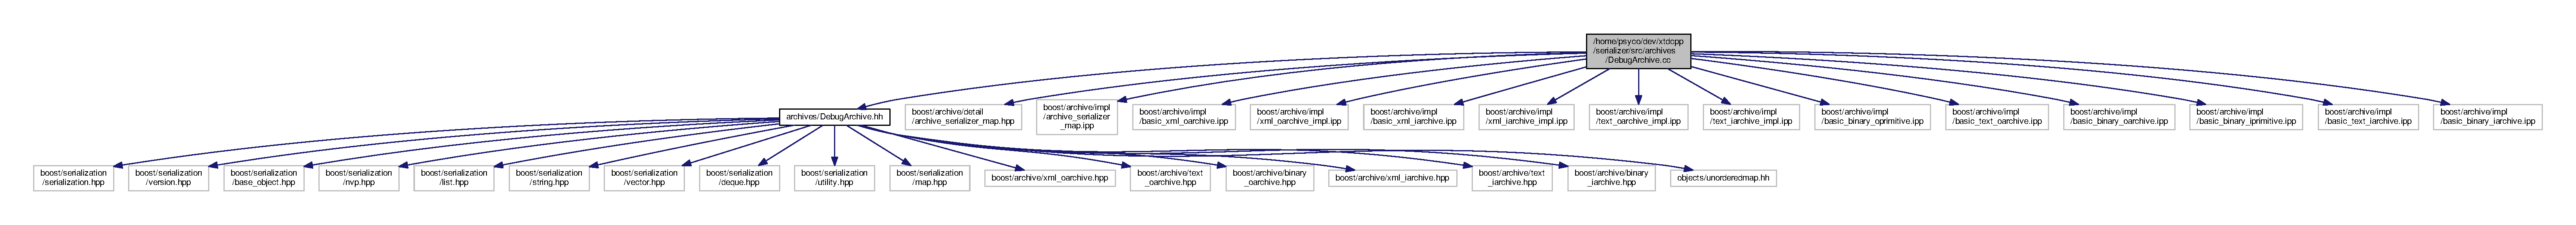
\includegraphics[width=350pt]{DebugArchive_8cc__incl}
\end{center}
\end{figure}
\subsection*{Namespaces}
\begin{DoxyCompactItemize}
\item 
\hyperlink{namespaceboost}{boost}
\item 
\hyperlink{namespaceboost_1_1archive}{boost\-::archive}
\end{DoxyCompactItemize}

\hypertarget{DebugArchive_8hh}{\section{/home/travis/build/psycofdj/xtdcpp/serializer/src/archives/\-Debug\-Archive.hh File Reference}
\label{DebugArchive_8hh}\index{/home/travis/build/psycofdj/xtdcpp/serializer/src/archives/\-Debug\-Archive.\-hh@{/home/travis/build/psycofdj/xtdcpp/serializer/src/archives/\-Debug\-Archive.\-hh}}
}
{\ttfamily \#include $<$boost/serialization/serialization.\-hpp$>$}\\*
{\ttfamily \#include $<$boost/serialization/version.\-hpp$>$}\\*
{\ttfamily \#include $<$boost/serialization/base\-\_\-object.\-hpp$>$}\\*
{\ttfamily \#include $<$boost/serialization/nvp.\-hpp$>$}\\*
{\ttfamily \#include $<$boost/serialization/list.\-hpp$>$}\\*
{\ttfamily \#include $<$boost/serialization/string.\-hpp$>$}\\*
{\ttfamily \#include $<$boost/serialization/vector.\-hpp$>$}\\*
{\ttfamily \#include $<$boost/serialization/deque.\-hpp$>$}\\*
{\ttfamily \#include $<$boost/serialization/utility.\-hpp$>$}\\*
{\ttfamily \#include $<$boost/serialization/map.\-hpp$>$}\\*
{\ttfamily \#include $<$boost/archive/xml\-\_\-oarchive.\-hpp$>$}\\*
{\ttfamily \#include $<$boost/archive/text\-\_\-oarchive.\-hpp$>$}\\*
{\ttfamily \#include $<$boost/archive/binary\-\_\-oarchive.\-hpp$>$}\\*
{\ttfamily \#include $<$boost/archive/xml\-\_\-iarchive.\-hpp$>$}\\*
{\ttfamily \#include $<$boost/archive/text\-\_\-iarchive.\-hpp$>$}\\*
{\ttfamily \#include $<$boost/archive/binary\-\_\-iarchive.\-hpp$>$}\\*
{\ttfamily \#include \char`\"{}objects/unorderedmap.\-hh\char`\"{}}\\*
Include dependency graph for Debug\-Archive.\-hh\-:
\nopagebreak
\begin{figure}[H]
\begin{center}
\leavevmode
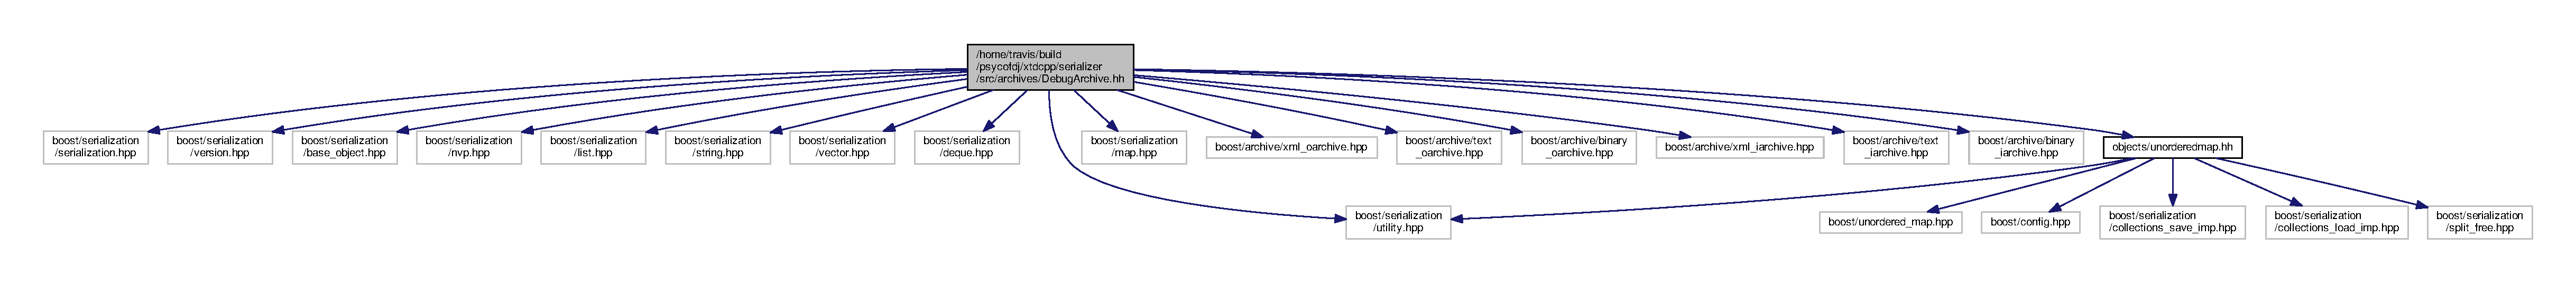
\includegraphics[width=350pt]{DebugArchive_8hh__incl}
\end{center}
\end{figure}
This graph shows which files directly or indirectly include this file\-:
\nopagebreak
\begin{figure}[H]
\begin{center}
\leavevmode
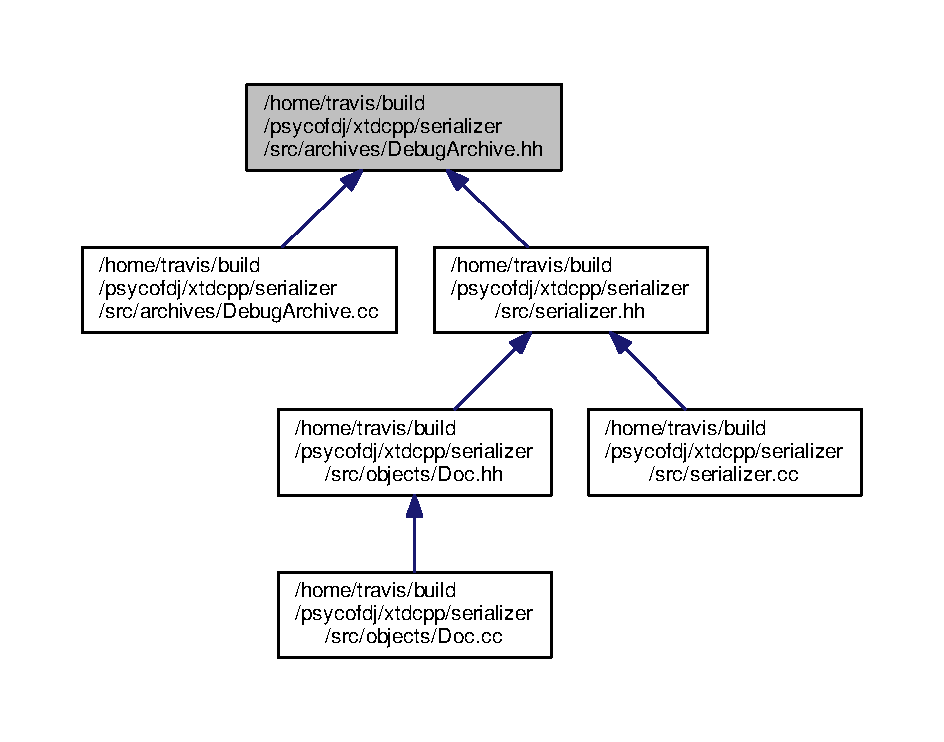
\includegraphics[width=350pt]{DebugArchive_8hh__dep__incl}
\end{center}
\end{figure}
\subsection*{Classes}
\begin{DoxyCompactItemize}
\item 
class \hyperlink{classxtd_1_1serializer_1_1DebugXmlOArchive}{xtd\-::serializer\-::\-Debug\-Xml\-O\-Archive}
\item 
class \hyperlink{classxtd_1_1serializer_1_1DebugXmlIArchive}{xtd\-::serializer\-::\-Debug\-Xml\-I\-Archive}
\item 
class \hyperlink{classxtd_1_1serializer_1_1DebugTextOArchive}{xtd\-::serializer\-::\-Debug\-Text\-O\-Archive}
\item 
class \hyperlink{classxtd_1_1serializer_1_1DebugTextIArchive}{xtd\-::serializer\-::\-Debug\-Text\-I\-Archive}
\item 
class \hyperlink{classxtd_1_1serializer_1_1DebugBinOArchive}{xtd\-::serializer\-::\-Debug\-Bin\-O\-Archive}
\item 
class \hyperlink{classxtd_1_1serializer_1_1DebugBinIArchive}{xtd\-::serializer\-::\-Debug\-Bin\-I\-Archive}
\end{DoxyCompactItemize}
\subsection*{Namespaces}
\begin{DoxyCompactItemize}
\item 
\hyperlink{namespacextd}{xtd}
\item 
\hyperlink{namespacextd_1_1serializer}{xtd\-::serializer}
\end{DoxyCompactItemize}

\hypertarget{Doc_8cc}{\section{/home/travis/build/psycofdj/xtdcpp/serializer/src/objects/\-Doc.cc File Reference}
\label{Doc_8cc}\index{/home/travis/build/psycofdj/xtdcpp/serializer/src/objects/\-Doc.\-cc@{/home/travis/build/psycofdj/xtdcpp/serializer/src/objects/\-Doc.\-cc}}
}
{\ttfamily \#include \char`\"{}objects/\-Doc.\-hh\char`\"{}}\\*
Include dependency graph for Doc.\-cc\-:
\nopagebreak
\begin{figure}[H]
\begin{center}
\leavevmode
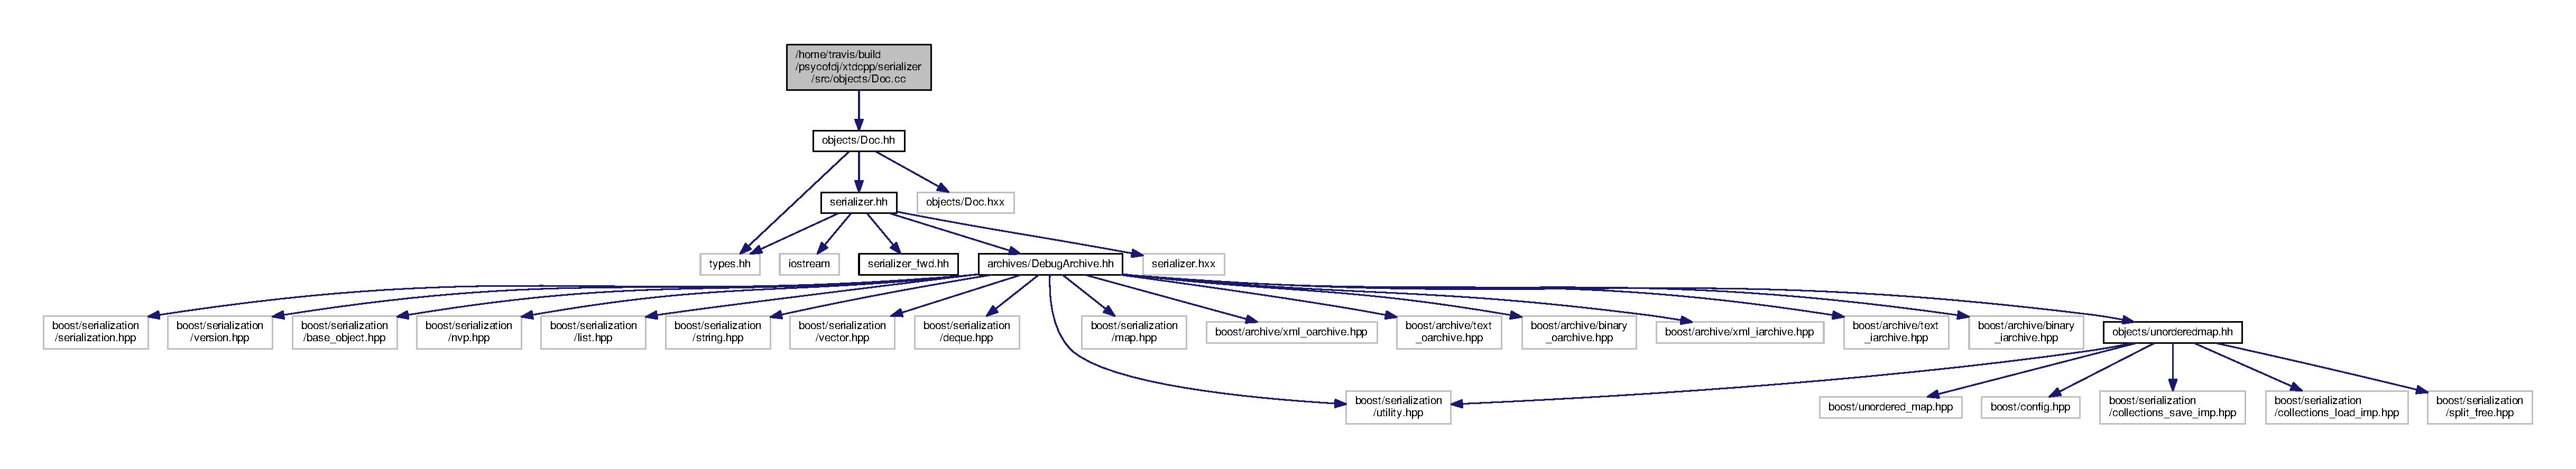
\includegraphics[width=350pt]{Doc_8cc__incl}
\end{center}
\end{figure}
\subsection*{Namespaces}
\begin{DoxyCompactItemize}
\item 
\hyperlink{namespacextd}{xtd}
\item 
\hyperlink{namespacextd_1_1serializer}{xtd\-::serializer}
\end{DoxyCompactItemize}

\hypertarget{Doc_8hh}{}\section{/home/psyco/dev/xtdcpp/serializer/src/objects/\+Doc.hh File Reference}
\label{Doc_8hh}\index{/home/psyco/dev/xtdcpp/serializer/src/objects/\+Doc.\+hh@{/home/psyco/dev/xtdcpp/serializer/src/objects/\+Doc.\+hh}}
{\ttfamily \#include $<$types.\+hh$>$}\\*
{\ttfamily \#include \char`\"{}serializer.\+hh\char`\"{}}\\*
{\ttfamily \#include \char`\"{}objects/\+Doc.\+hxx\char`\"{}}\\*
Include dependency graph for Doc.\+hh\+:
\nopagebreak
\begin{figure}[H]
\begin{center}
\leavevmode
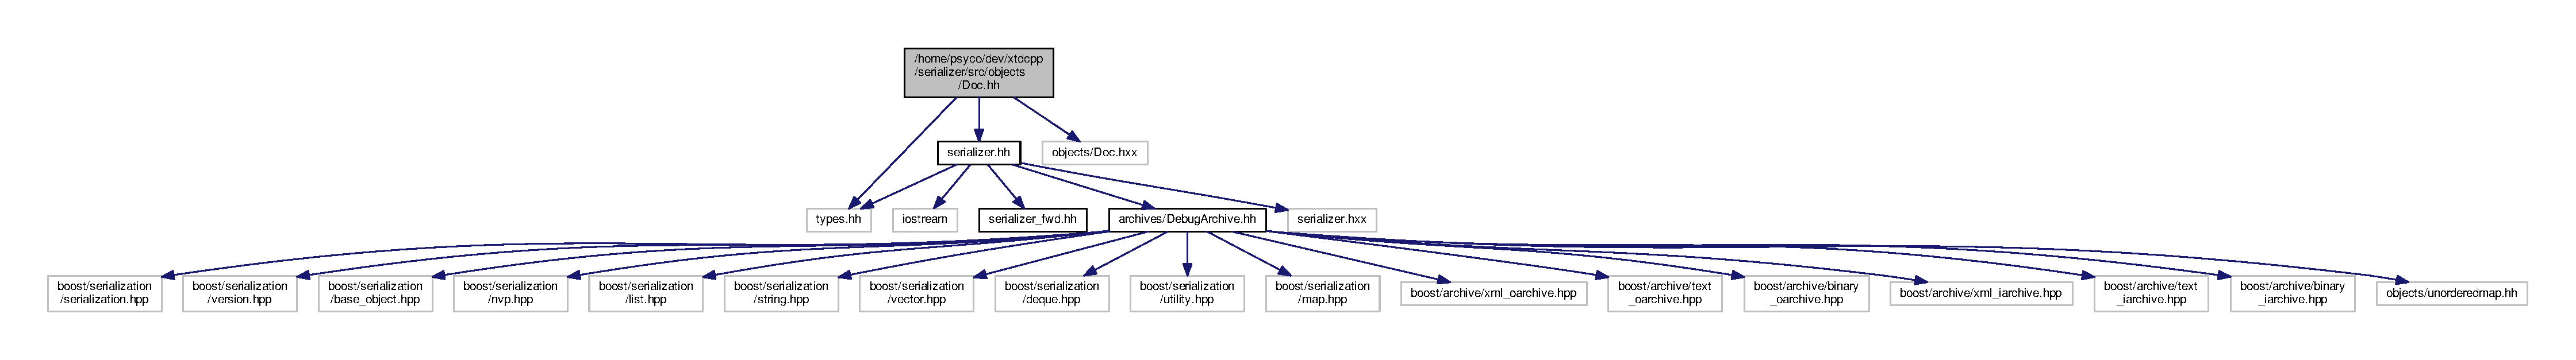
\includegraphics[width=350pt]{Doc_8hh__incl}
\end{center}
\end{figure}
This graph shows which files directly or indirectly include this file\+:
\nopagebreak
\begin{figure}[H]
\begin{center}
\leavevmode
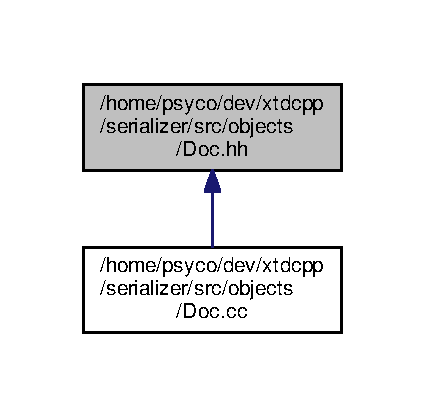
\includegraphics[width=204pt]{Doc_8hh__dep__incl}
\end{center}
\end{figure}
\subsection*{Classes}
\begin{DoxyCompactItemize}
\item 
class \hyperlink{classxtd_1_1serializer_1_1Doc}{xtd\+::serializer\+::\+Doc}
\end{DoxyCompactItemize}
\subsection*{Namespaces}
\begin{DoxyCompactItemize}
\item 
 \hyperlink{namespacextd}{xtd}
\item 
 \hyperlink{namespacextd_1_1serializer}{xtd\+::serializer}
\end{DoxyCompactItemize}

\hypertarget{serializer_8cc}{}\section{/home/psyco/dev/xtdcpp/serializer/src/serializer.cc File Reference}
\label{serializer_8cc}\index{/home/psyco/dev/xtdcpp/serializer/src/serializer.\+cc@{/home/psyco/dev/xtdcpp/serializer/src/serializer.\+cc}}
{\ttfamily \#include \char`\"{}serializer.\+hh\char`\"{}}\\*
Include dependency graph for serializer.\+cc\+:
\nopagebreak
\begin{figure}[H]
\begin{center}
\leavevmode
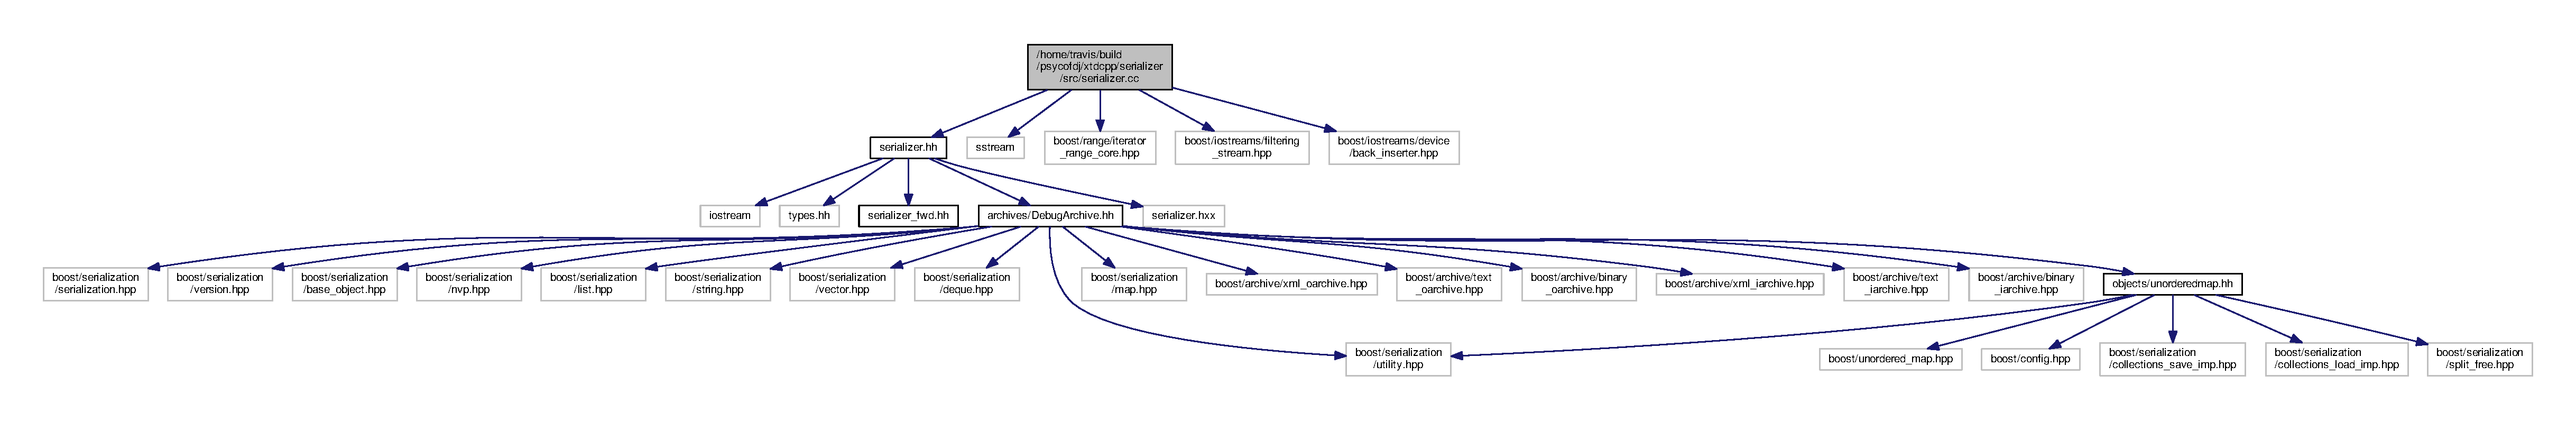
\includegraphics[width=350pt]{serializer_8cc__incl}
\end{center}
\end{figure}
\subsection*{Namespaces}
\begin{DoxyCompactItemize}
\item 
 \hyperlink{namespacextd}{xtd}
\item 
 \hyperlink{namespacextd_1_1serializer}{xtd\+::serializer}
\end{DoxyCompactItemize}

\hypertarget{serializer_8hh}{}\section{/home/psyco/dev/xtdcpp/serializer/src/serializer.hh File Reference}
\label{serializer_8hh}\index{/home/psyco/dev/xtdcpp/serializer/src/serializer.\+hh@{/home/psyco/dev/xtdcpp/serializer/src/serializer.\+hh}}
{\ttfamily \#include $<$iostream$>$}\\*
{\ttfamily \#include $<$types.\+hh$>$}\\*
{\ttfamily \#include \char`\"{}serializer\+\_\+fwd.\+hh\char`\"{}}\\*
{\ttfamily \#include \char`\"{}archives/\+Debug\+Archive.\+hh\char`\"{}}\\*
{\ttfamily \#include \char`\"{}serializer.\+hxx\char`\"{}}\\*
Include dependency graph for serializer.\+hh\+:
\nopagebreak
\begin{figure}[H]
\begin{center}
\leavevmode
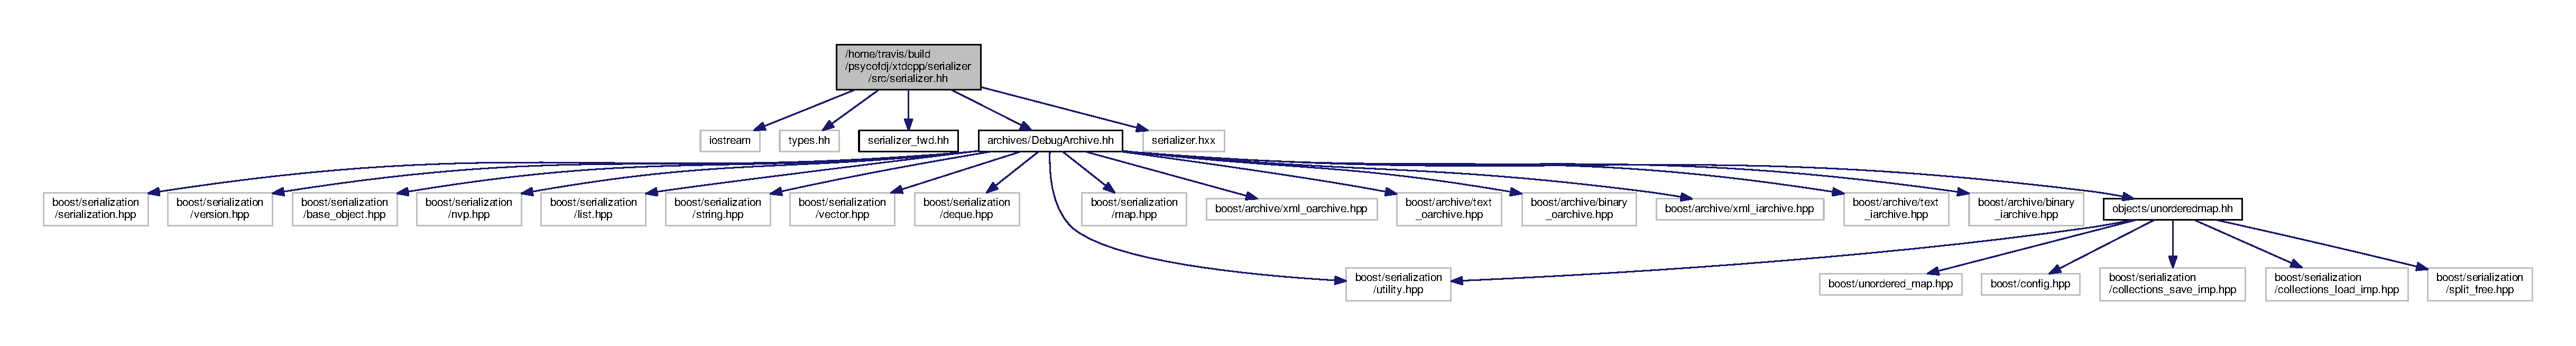
\includegraphics[width=350pt]{serializer_8hh__incl}
\end{center}
\end{figure}
This graph shows which files directly or indirectly include this file\+:
\nopagebreak
\begin{figure}[H]
\begin{center}
\leavevmode
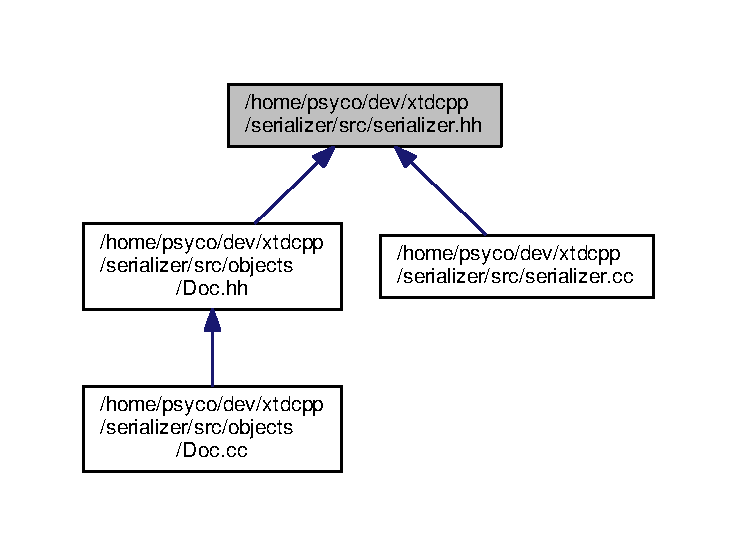
\includegraphics[width=350pt]{serializer_8hh__dep__incl}
\end{center}
\end{figure}
\subsection*{Classes}
\begin{DoxyCompactItemize}
\item 
struct \hyperlink{structxtd_1_1serializer_1_1mode}{xtd\+::serializer\+::mode}
\item 
struct \hyperlink{structxtd_1_1serializer_1_1mode_1_1text}{xtd\+::serializer\+::mode\+::text}
\item 
struct \hyperlink{structxtd_1_1serializer_1_1mode_1_1xml}{xtd\+::serializer\+::mode\+::xml}
\item 
struct \hyperlink{structxtd_1_1serializer_1_1mode_1_1bin}{xtd\+::serializer\+::mode\+::bin}
\item 
struct \hyperlink{structxtd_1_1serializer_1_1option}{xtd\+::serializer\+::option}
\item 
struct \hyperlink{structxtd_1_1serializer_1_1serializer}{xtd\+::serializer\+::serializer$<$ Mode $>$}
\end{DoxyCompactItemize}
\subsection*{Namespaces}
\begin{DoxyCompactItemize}
\item 
 \hyperlink{namespacextd}{xtd}
\item 
 \hyperlink{namespacextd_1_1serializer}{xtd\+::serializer}
\end{DoxyCompactItemize}
\subsection*{Macros}
\begin{DoxyCompactItemize}
\item 
\#define \hyperlink{serializer_8hh_a54ebd30f6967d7f47176460bf889311b}{E\+N\+U\+M\+\_\+\+C\+A\+SE}(p\+\_\+value,  p\+\_\+dst)
\end{DoxyCompactItemize}
\subsection*{Functions}
\begin{DoxyCompactItemize}
\item 
{\footnotesize template$<$class T $>$ }\\string \hyperlink{namespacextd_1_1serializer_aff0b24f230c8b5083104eccb94242a8c}{xtd\+::serializer\+::as\+\_\+xml} (const T \&p\+\_\+obj, bool p\+\_\+debug, option p\+\_\+opt=option())
\item 
{\footnotesize template$<$class T $>$ }\\std\+::vector$<$ char $>$ \hyperlink{namespacextd_1_1serializer_a0088e6d509f6652e58c7c0eea9102884}{xtd\+::serializer\+::as\+\_\+bin} (const T \&p\+\_\+obj, bool p\+\_\+debug, option p\+\_\+opt=option())
\item 
{\footnotesize template$<$class T $>$ }\\void \hyperlink{namespacextd_1_1serializer_a1c43eba643505bba5858d6d5431201fb}{xtd\+::serializer\+::as\+\_\+bin} (const T \&p\+\_\+obj, std\+::vector$<$ char $>$ \&p\+\_\+data, bool p\+\_\+debug, option p\+\_\+opt=option())
\item 
{\footnotesize template$<$class T $>$ }\\std\+::vector$<$ char $>$ \hyperlink{namespacextd_1_1serializer_a5ac463bb961b98f1b8b7c2655d2772db}{xtd\+::serializer\+::as\+\_\+text} (const T \&p\+\_\+obj, bool p\+\_\+debug, option p\+\_\+opt=option())
\item 
{\footnotesize template$<$class T $>$ }\\void \hyperlink{namespacextd_1_1serializer_a601beccda10ec2760c371d39045bec0e}{xtd\+::serializer\+::from\+\_\+bin} (const std\+::vector$<$ char $>$ \&p\+\_\+data, T \&p\+\_\+obj, option p\+\_\+opt=option())
\item 
{\footnotesize template$<$class T $>$ }\\void \hyperlink{namespacextd_1_1serializer_a76ec6ed068121fc7ff0f6514132c5683}{xtd\+::serializer\+::from\+\_\+bin} (const std\+::vector$<$ char $>$ \&p\+\_\+data, T \&p\+\_\+obj, bool \&p\+\_\+debug, option p\+\_\+opt=option())
\item 
{\footnotesize template$<$class T $>$ }\\void \hyperlink{namespacextd_1_1serializer_a27ea640a20bff130274562ddd8762c0a}{xtd\+::serializer\+::from\+\_\+text} (const std\+::vector$<$ char $>$ \&p\+\_\+data, T \&p\+\_\+obj, bool \&p\+\_\+debug, option p\+\_\+opt=option())
\end{DoxyCompactItemize}


\subsection{Macro Definition Documentation}
\index{serializer.\+hh@{serializer.\+hh}!E\+N\+U\+M\+\_\+\+C\+A\+SE@{E\+N\+U\+M\+\_\+\+C\+A\+SE}}
\index{E\+N\+U\+M\+\_\+\+C\+A\+SE@{E\+N\+U\+M\+\_\+\+C\+A\+SE}!serializer.\+hh@{serializer.\+hh}}
\subsubsection[{\texorpdfstring{E\+N\+U\+M\+\_\+\+C\+A\+SE}{ENUM_CASE}}]{\setlength{\rightskip}{0pt plus 5cm}\#define E\+N\+U\+M\+\_\+\+C\+A\+SE(
\begin{DoxyParamCaption}
\item[{}]{p\+\_\+value, }
\item[{}]{p\+\_\+dst}
\end{DoxyParamCaption}
)}\hypertarget{serializer_8hh_a54ebd30f6967d7f47176460bf889311b}{}\label{serializer_8hh_a54ebd30f6967d7f47176460bf889311b}
{\bfseries Value\+:}
\begin{DoxyCode}
\textcolor{keywordflow}{case} p\_value :                                \(\backslash\)
  p\_dst = #p\_value;                             \(\backslash\)
  break;
\end{DoxyCode}


Definition at line 12 of file serializer.\+hh.


\hypertarget{serializer__fwd_8hh}{\section{/home/travis/build/psycofdj/xtdcpp/serializer/src/serializer\-\_\-fwd.hh File Reference}
\label{serializer__fwd_8hh}\index{/home/travis/build/psycofdj/xtdcpp/serializer/src/serializer\-\_\-fwd.\-hh@{/home/travis/build/psycofdj/xtdcpp/serializer/src/serializer\-\_\-fwd.\-hh}}
}
This graph shows which files directly or indirectly include this file\-:
\nopagebreak
\begin{figure}[H]
\begin{center}
\leavevmode
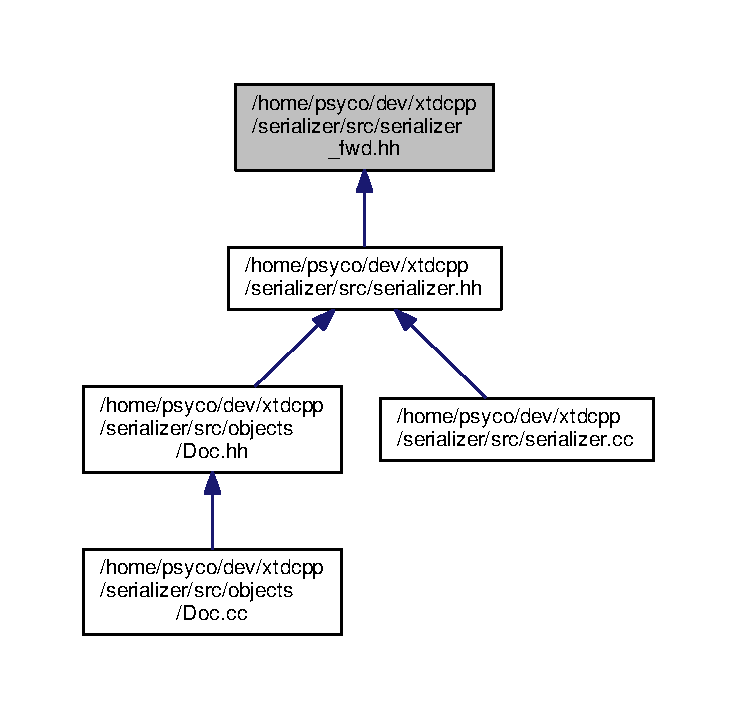
\includegraphics[width=350pt]{serializer__fwd_8hh__dep__incl}
\end{center}
\end{figure}
\subsection*{Namespaces}
\begin{DoxyCompactItemize}
\item 
\hyperlink{namespacextd}{xtd}
\item 
\hyperlink{namespacextd_1_1serializer}{xtd\-::serializer}
\end{DoxyCompactItemize}

%--- End generated contents ---

% Index
\backmatter
\newpage
\phantomsection
\clearemptydoublepage
\addcontentsline{toc}{chapter}{Index}
\printindex

\end{document}
